
\begin{landscape}
{\footnotesize
\begin{longtable}{|p{0.11\textwidth}|p{0.09\textwidth}|p{0.07\textwidth}|p{0.07\textwidth}|p{0.09\textwidth}|p{0.11\textwidth}|p{0.11\textwidth}|p{0.11\textwidth}|p{0.07\textwidth}|p{0.07\textwidth}|p{0.04\textwidth}|p{0.04\textwidth}|}
\hline
\textbf{Ratings} & \textbf{Name} & \textbf{Domain} & \textbf{Focus} & \textbf{Keywords} & \textbf{Task Types} & \textbf{AI/ML Motif} & \textbf{AI Capability} & \textbf{Metrics} & \textbf{Models} & \textbf{Average Rating} & \textbf{Citation}  \\ \hline
\endfirsthead
\hline
\textbf{Ratings} & \textbf{Name} & \textbf{Domain} & \textbf{Focus} & \textbf{Keywords} & \textbf{Task Types} & \textbf{AI/ML Motif} & \textbf{AI Capability} & \textbf{Metrics} & \textbf{Models} & \textbf{Average Rating} & \textbf{Citation}  \\ \hline
\endhead
\hline
\multicolumn{12}{r}{Continued on next page} \\
\endfoot
\hline
\endlastfoot
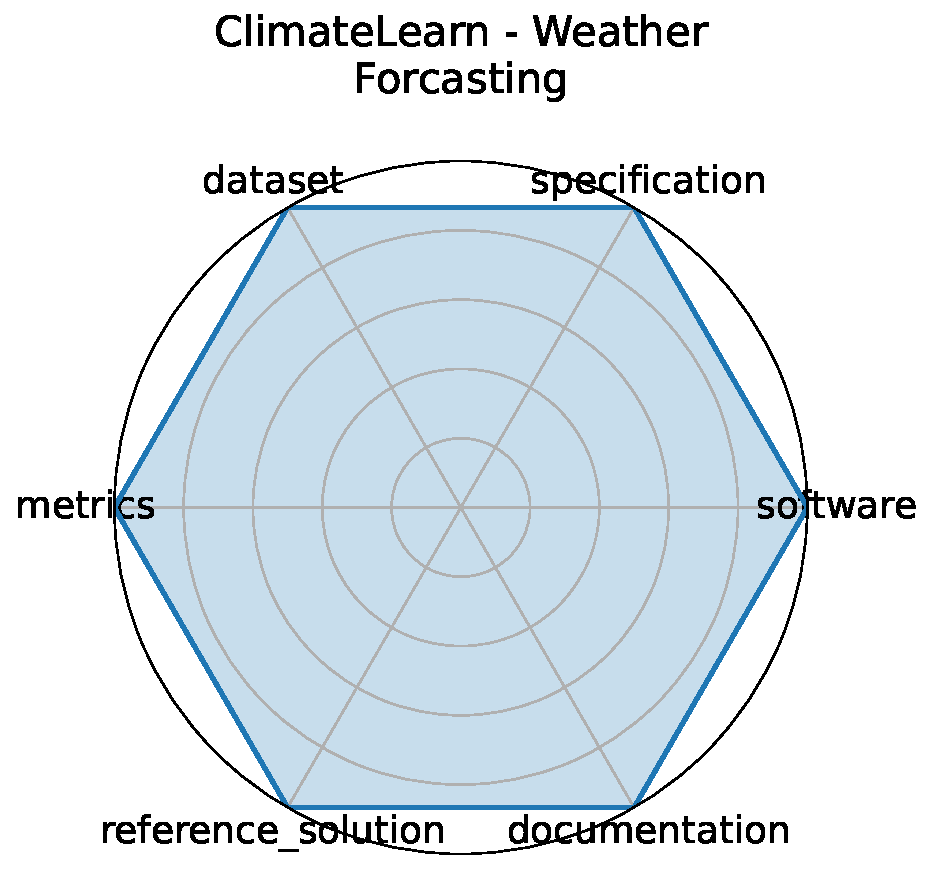
\includegraphics[width=0.15\textwidth]{climatelearn_-_weather_forcasting_radar.pdf} & ClimateLearn - Weather Forcasting & Climate \& Earth Science & ML for weather and climate modeling & medium-range forecasting, ERA5, data-driven & Forecasting & Sequence Prediction/Forecasting & Global weather prediction (3-5 days) & RMSE, Anomaly correlation & CNN baselines, ResNet variants & \textbf{5.00} & \cite{nguyen2023climatelearnbenchmarkingmachinelearning} \\ \hline
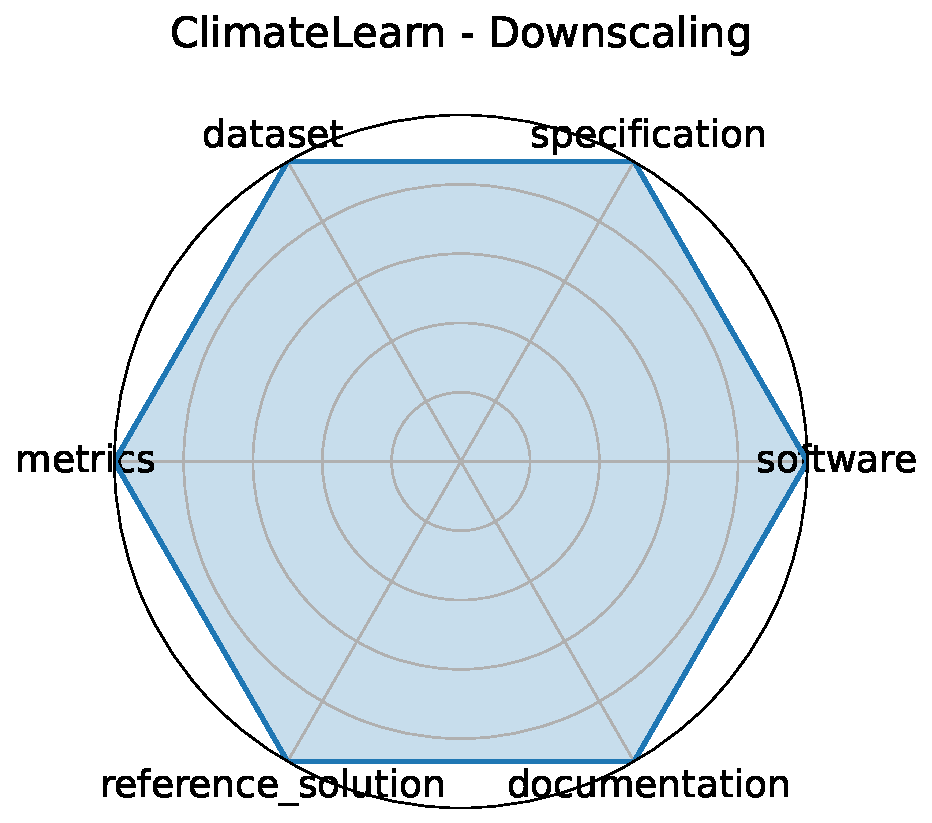
\includegraphics[width=0.15\textwidth]{climatelearn_-_downscaling_radar.pdf} & ClimateLearn - Downscaling & Climate \& Earth Science & ML for weather and climate modeling & medium-range forecasting, ERA5, data-driven & Forecasting & Regression & Global weather prediction (3-5 days) & RMSE, Anomaly correlation & CNN baselines, ResNet variants & \textbf{5.00} & \cite{nguyen2023climatelearnbenchmarkingmachinelearning} \\ \hline
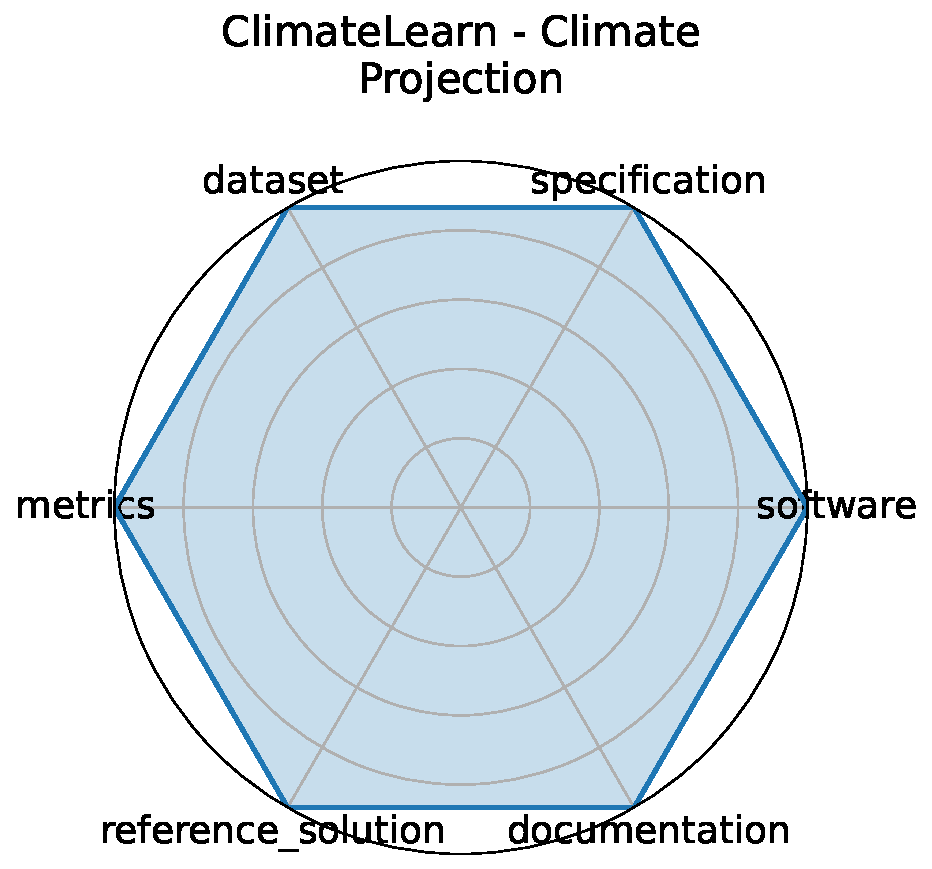
\includegraphics[width=0.15\textwidth]{climatelearn_-_climate_projection_radar.pdf} & ClimateLearn - Climate Projection & Climate \& Earth Science & ML for weather and climate modeling & medium-range forecasting, ERA5, data-driven & Forecasting & Regression & Global weather prediction (3-5 days) & RMSE, Anomaly correlation & CNN baselines, ResNet variants & \textbf{5.00} & \cite{nguyen2023climatelearnbenchmarkingmachinelearning} \\ \hline
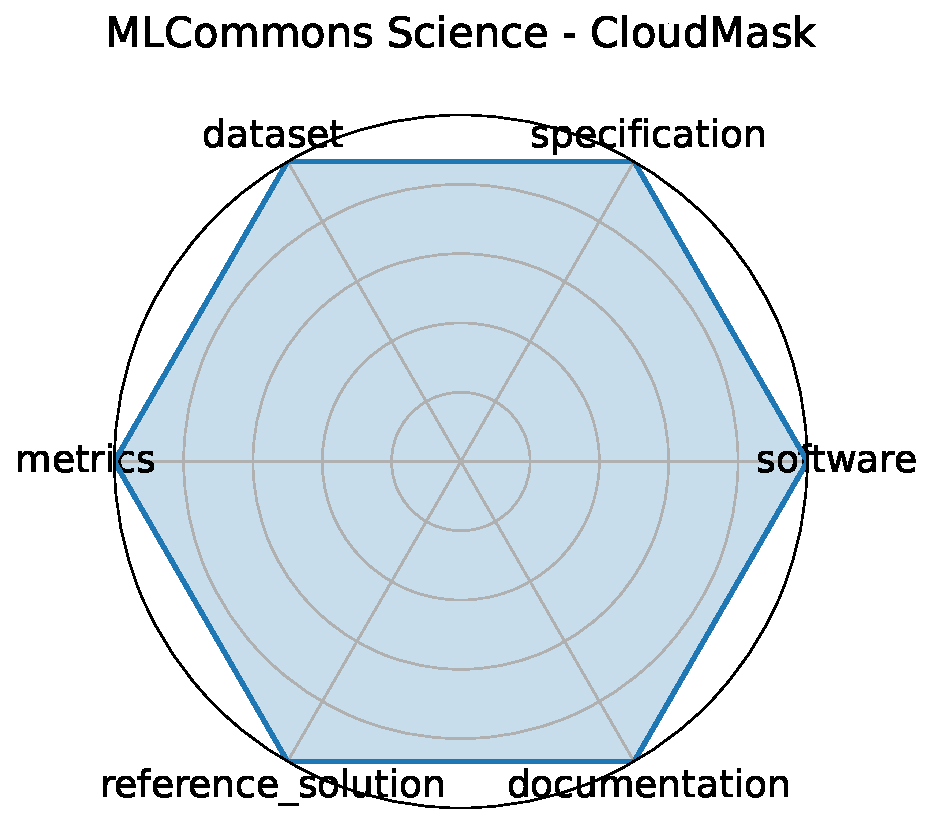
\includegraphics[width=0.15\textwidth]{mlcommons_science_-_cloudmask_radar.pdf} & MLCommons Science - CloudMask & Climate \& Earth Science & AI benchmarks for scientific applications including time-series, imaging, and simulation & science AI, benchmark, MLCommons, HPC & Time-series analysis, Image classification, Simulation surrogate modeling & Classification & Inference accuracy, simulation speed-up, generalization & MAE, Accuracy, Speedup vs simulation & CNN, GNN, Transformer & \textbf{5.00} & \cite{10.1007/978-3-031-23220-6_4} \\ \hline
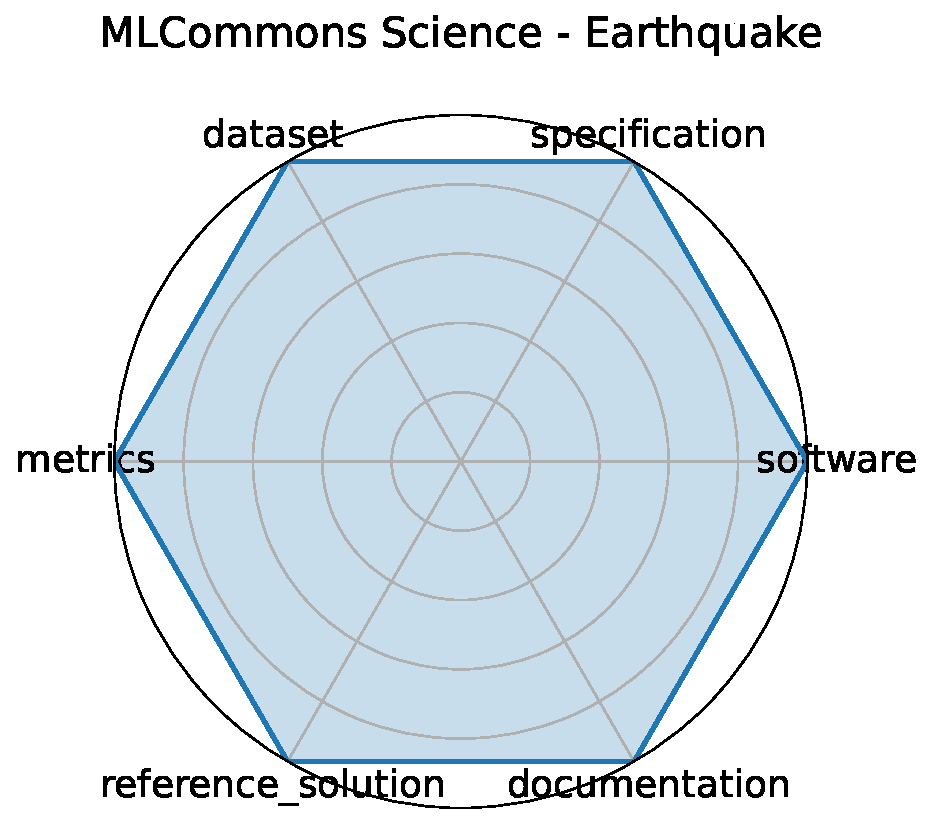
\includegraphics[width=0.15\textwidth]{mlcommons_science_-_earthquake_radar.pdf} & MLCommons Science - Earthquake & Climate \& Earth Science & AI benchmarks for scientific applications including time-series, imaging, and simulation & science AI, benchmark, MLCommons, HPC & Time-series analysis, Image classification, Simulation surrogate modeling & Sequence Prediction/Forecasting & Inference accuracy, simulation speed-up, generalization & MAE, Accuracy, Speedup vs simulation & CNN, GNN, Transformer & \textbf{5.00} & \cite{10.1007/978-3-031-23220-6_4} \\ \hline
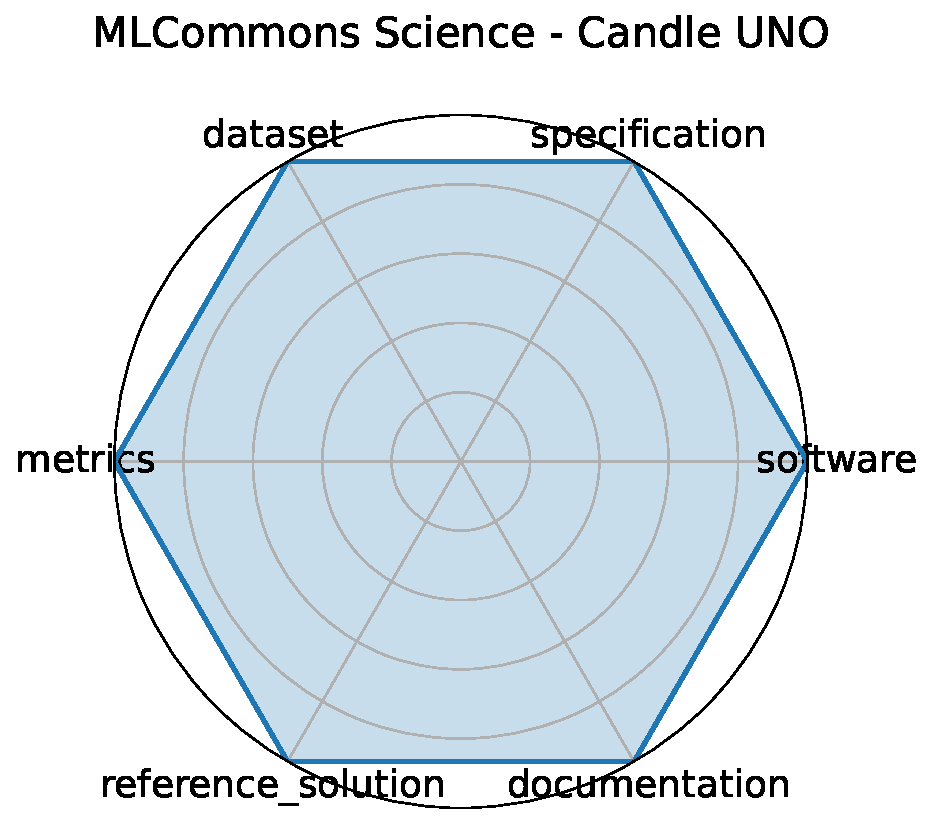
\includegraphics[width=0.15\textwidth]{mlcommons_science_-_candle_uno_radar.pdf} & MLCommons Science - Candle UNO & Biology \& Medicine & AI benchmarks for scientific applications including time-series, imaging, and simulation & science AI, benchmark, MLCommons, HPC & Time-series analysis, Image classification, Simulation surrogate modeling & Classification & Inference accuracy, simulation speed-up, generalization & MAE, Accuracy, Speedup vs simulation & CNN, GNN, Transformer & \textbf{5.00} & \cite{10.1007/978-3-031-23220-6_4} \\ \hline
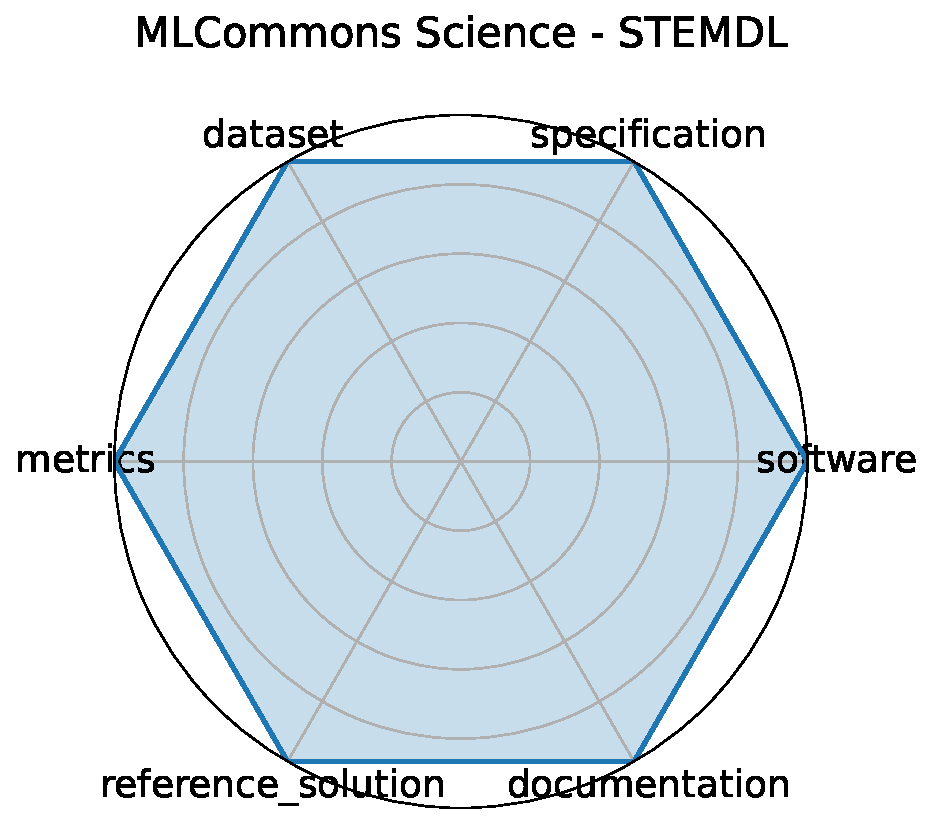
\includegraphics[width=0.15\textwidth]{mlcommons_science_-_stemdl_radar.pdf} & MLCommons Science - STEMDL & Materials Science & AI benchmarks for scientific applications including time-series, imaging, and simulation & science AI, benchmark, MLCommons, HPC & Time-series analysis, Image classification, Simulation surrogate modeling & Classification & Inference accuracy, simulation speed-up, generalization & MAE, Accuracy, Speedup vs simulation & CNN, GNN, Transformer & \textbf{5.00} & \cite{10.1007/978-3-031-23220-6_4} \\ \hline
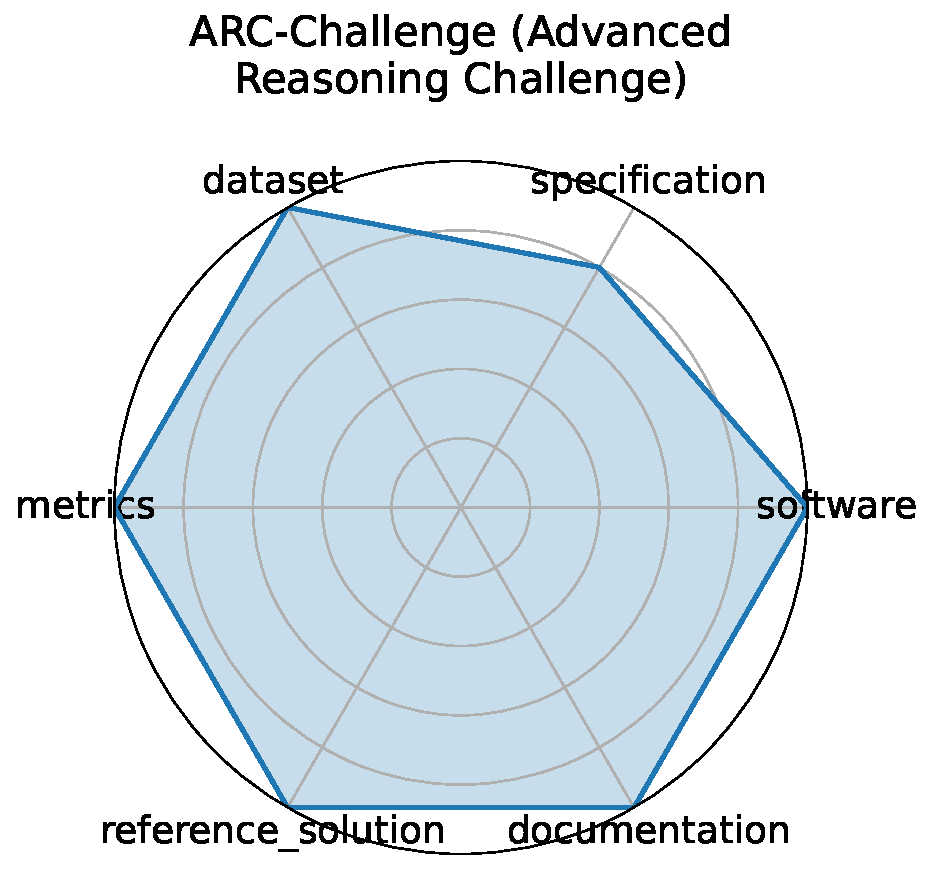
\includegraphics[width=0.15\textwidth]{arc-challenge_advanced_reasoning_challenge_radar.pdf} & ARC-Challenge (Advanced Reasoning Challenge) & Computational Science \& AI & Grade-school science with reasoning emphasis & grade-school, science QA, challenge set, reasoning & Multiple choice & Reasoning \& Generalization & Commonsense and scientific reasoning & Accuracy & GPT-4, Claude & \textbf{4.83} & \cite{allenai:arc} \\ \hline
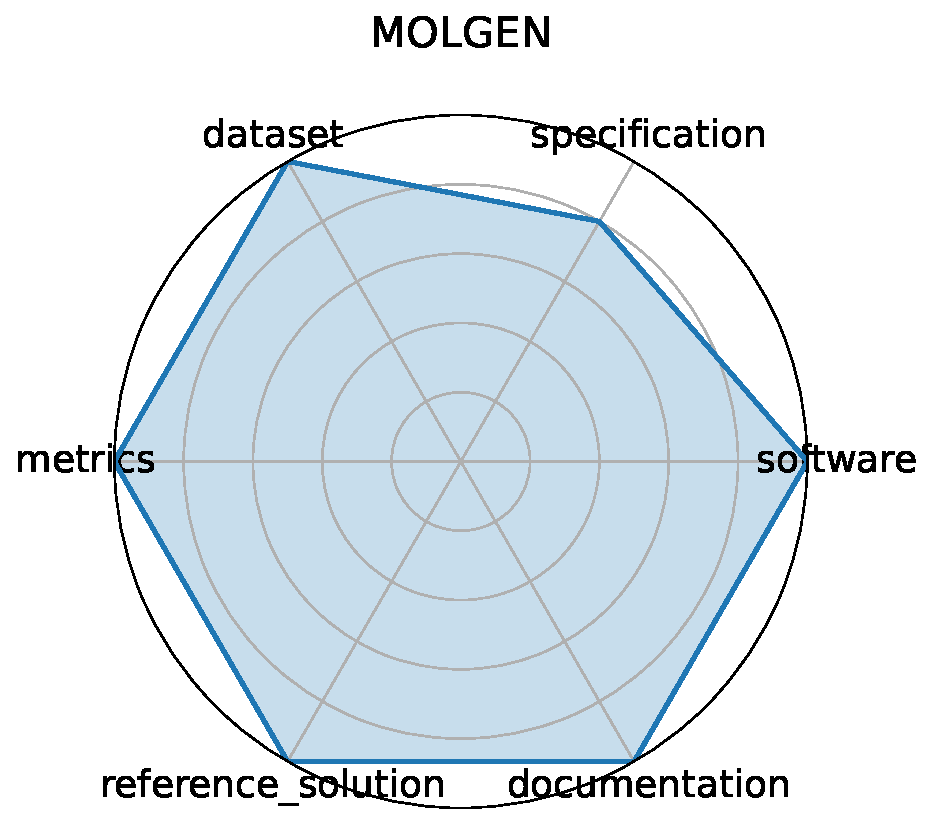
\includegraphics[width=0.15\textwidth]{molgen_radar.pdf} & MOLGEN & Chemistry & Molecular generation and optimization & SELFIES, GAN, property optimization & Distribution learning, Goal-oriented generation & Generative & Generation of valid and optimized molecular structures & Validity\%, Novelty\%, QED, Docking score, penalized logP & MolGen & \textbf{4.83} & \cite{fang2024domainagnosticmoleculargenerationchemical} \\ \hline
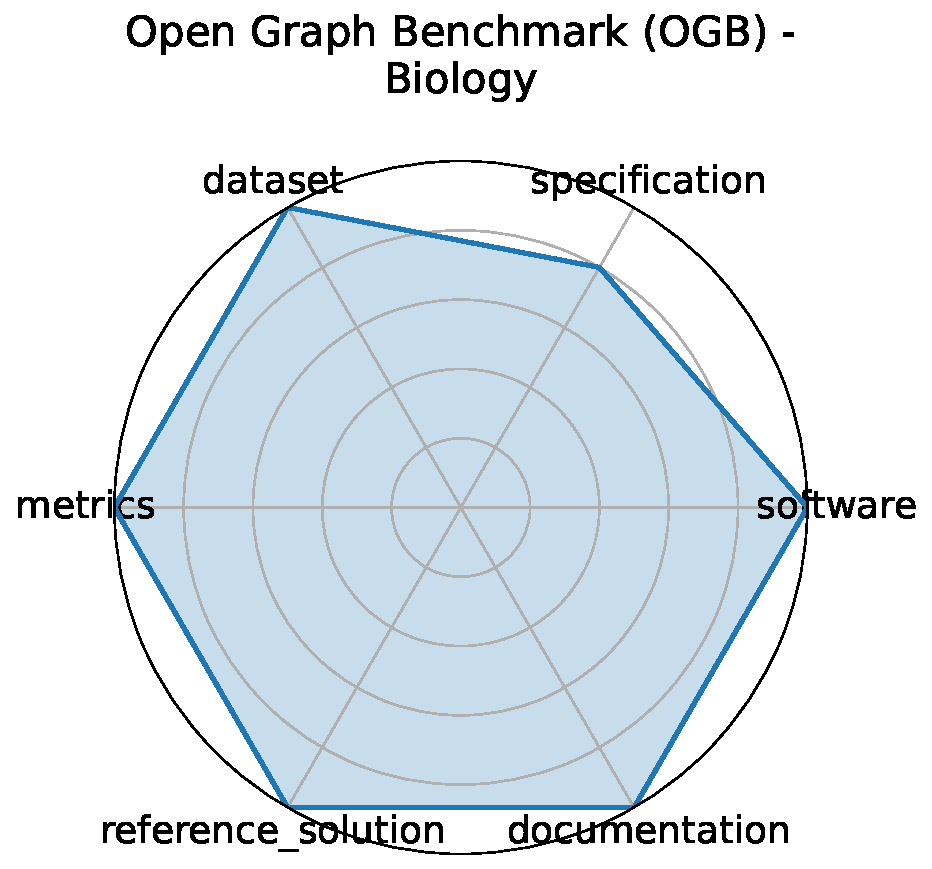
\includegraphics[width=0.15\textwidth]{open_graph_benchmark_ogb_-_biology_radar.pdf} & Open Graph Benchmark (OGB) - Biology & Biology \& Medicine & Biological graph property prediction & node prediction, link prediction, graph classification & Node property prediction, Link property prediction, Graph property prediction & Sequence Prediction/Forecasting & Scalability and generalization in graph ML for biology & Accuracy, ROC-AUC & GCN, GraphSAGE, GAT & \textbf{4.83} & \cite{hu2021opengraphbenchmarkdatasets} \\ \hline
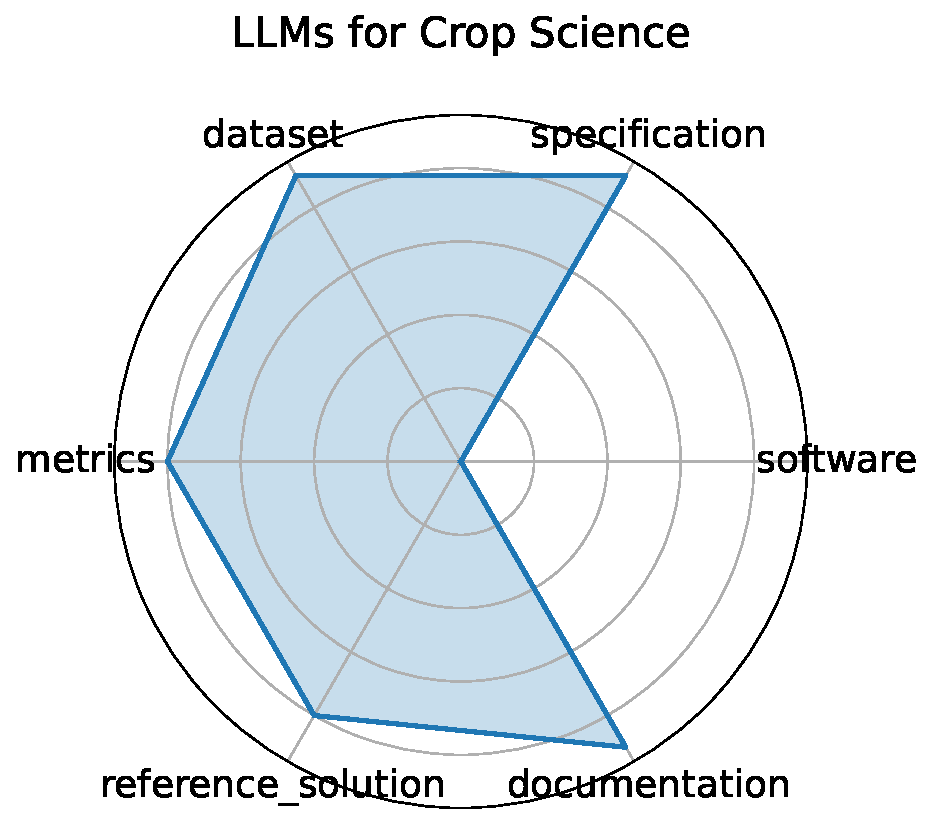
\includegraphics[width=0.15\textwidth]{llms_for_crop_science_radar.pdf} & LLMs for Crop Science & Climate \& Earth Science & Evaluating LLMs on crop trait QA and textual inference tasks with domain-specific prompts & crop science, prompt engineering, domain adaptation, question answering & Question Answering, Inference & Reasoning \& Generalization & Scientific knowledge, crop reasoning & Accuracy, F1 score & GPT-3.5, GPT-4, Claude-3-opus, Qwen-max, LLama3-8B, InternLM2-7B, Qwen1.5-7B & \textbf{4.67} & \cite{zhang2024empowering} \\ \hline
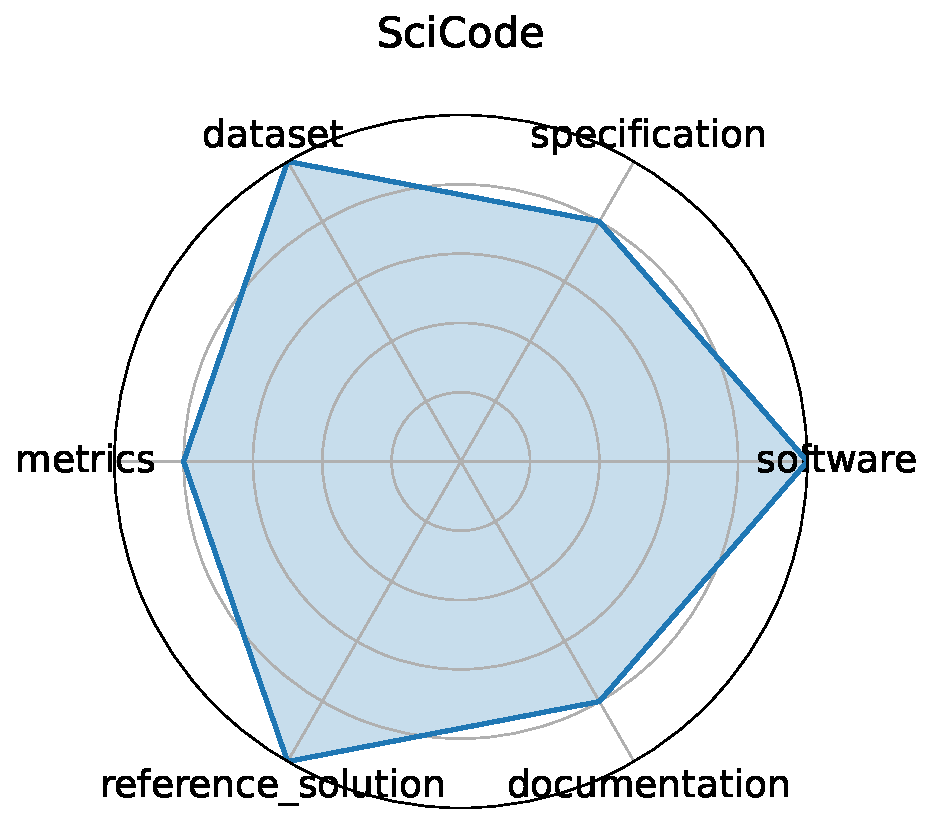
\includegraphics[width=0.15\textwidth]{scicode_radar.pdf} & SciCode & Computational Science \& AI & Scientific code generation and problem solving & code synthesis, scientific computing, programming benchmark & Coding & Generative & Program synthesis, scientific computing & Solve rate (\%) & Claude3.5-Sonnet & \textbf{4.50} & \cite{tian2024scicoderesearchcodingbenchmark} \\ \hline
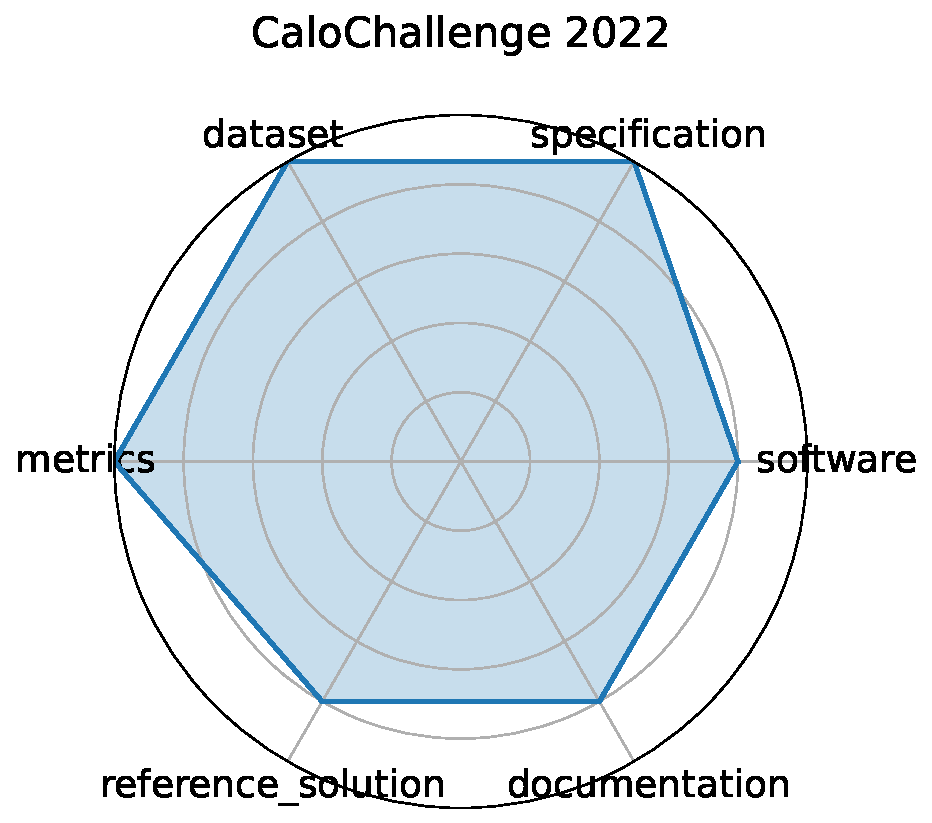
\includegraphics[width=0.15\textwidth]{calochallenge__radar.pdf} & CaloChallenge 2022 & High Energy Physics & Fast generative-model-based calorimeter shower simulation evaluation & calorimeter simulation, generative models, surrogate modeling, LHC, fast simulation & Surrogate modeling & Generative & Simulation fidelity, speed, efficiency & Histogram similarity, Classifier AUC, Generation latency & VAE variants, GAN variants, Normalizing flows, Diffusion models & \textbf{4.50} & \cite{krause2024calochallenge2022communitychallenge} \\ \hline
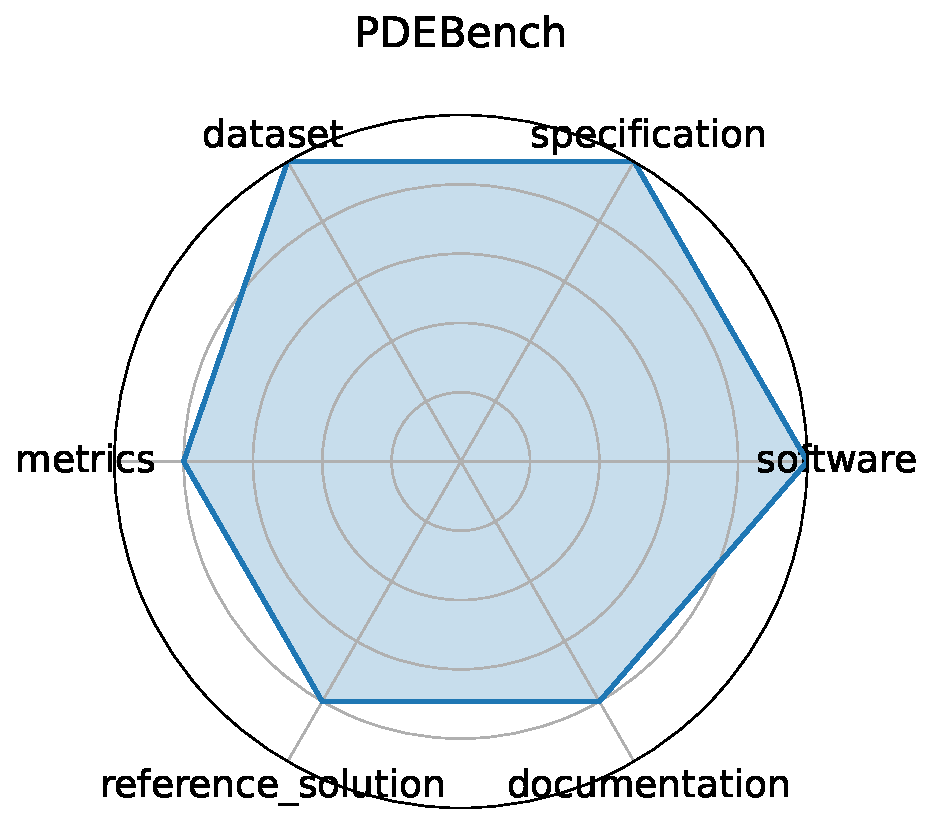
\includegraphics[width=0.15\textwidth]{pdebench_radar.pdf} & PDEBench & Computational Science \& AI, Climate \& Earth Science, Mathematics & Benchmark suite for ML-based surrogates solving time-dependent PDEs & PDEs, CFD, scientific ML, surrogate modeling, NeurIPS & Supervised Learning & Regression & Time-dependent PDE modeling; physical accuracy & RMSE, boundary RMSE, Fourier RMSE & FNO, U-Net, PINN, Gradient-Based inverse methods & \textbf{4.50} & \cite{takamoto2024pdebenchextensivebenchmarkscientific} \\ \hline
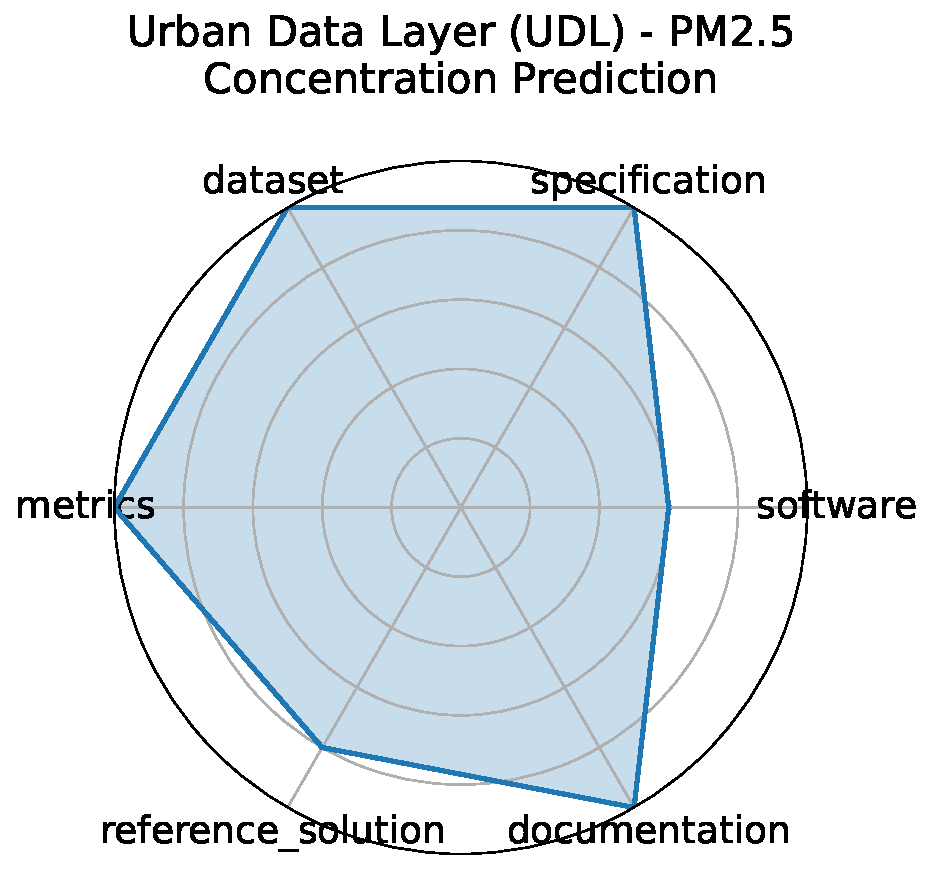
\includegraphics[width=0.15\textwidth]{urban_data_layer_udl_-_pm_concentration_prediction_radar.pdf} & Urban Data Layer (UDL) - PM2.5 Concentration Prediction & Climate \& Earth Science & Unified data pipeline for multi-modal urban science research & data pipeline, urban science, multi-modal, benchmark & Prediction, Classification & Regression & Multi-modal urban inference, standardization & Task-specific accuracy or RMSE & Baseline regression/classification pipelines & \textbf{4.50} & \cite{neurips2024_0db7f135} \\ \hline
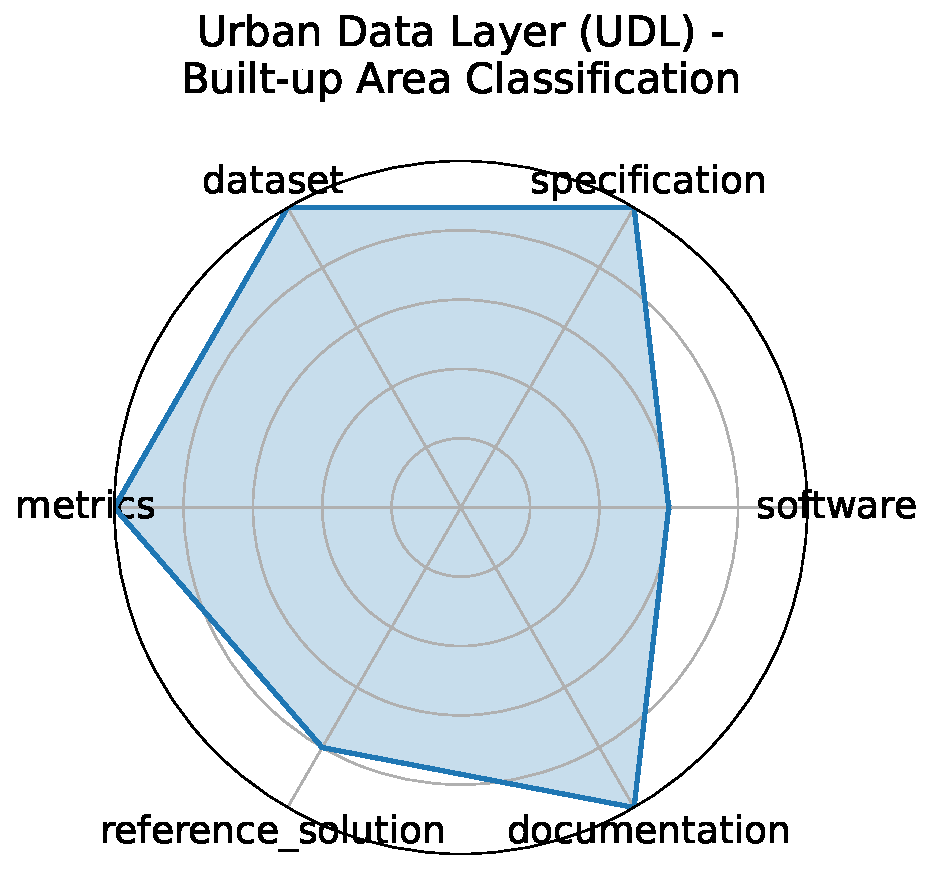
\includegraphics[width=0.15\textwidth]{urban_data_layer_udl_-_built-up_area_classification_radar.pdf} & Urban Data Layer (UDL) - Built-up Area Classification & Climate \& Earth Science & Unified data pipeline for multi-modal urban science research & data pipeline, urban science, multi-modal, benchmark & Prediction, Classification & Classification & Multi-modal urban inference, standardization & Task-specific accuracy or RMSE & Baseline regression/classification pipelines & \textbf{4.50} & \cite{neurips2024_0db7f135} \\ \hline
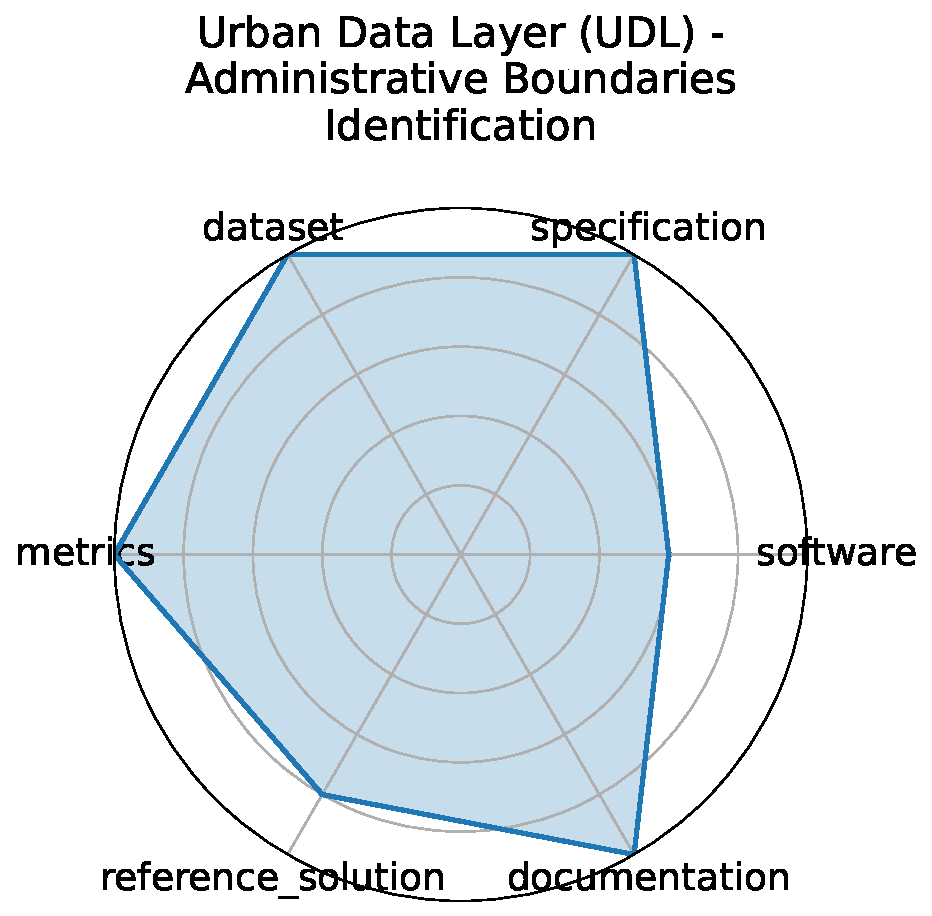
\includegraphics[width=0.15\textwidth]{urban_data_layer_udl_-_administrative_boundaries_identification_radar.pdf} & Urban Data Layer (UDL) - Administrative Boundaries Identification & Climate \& Earth Science & Unified data pipeline for multi-modal urban science research & data pipeline, urban science, multi-modal, benchmark & Prediction, Classification & Classification & Multi-modal urban inference, standardization & Task-specific accuracy or RMSE & Baseline regression/classification pipelines & \textbf{4.50} & \cite{neurips2024_0db7f135} \\ \hline
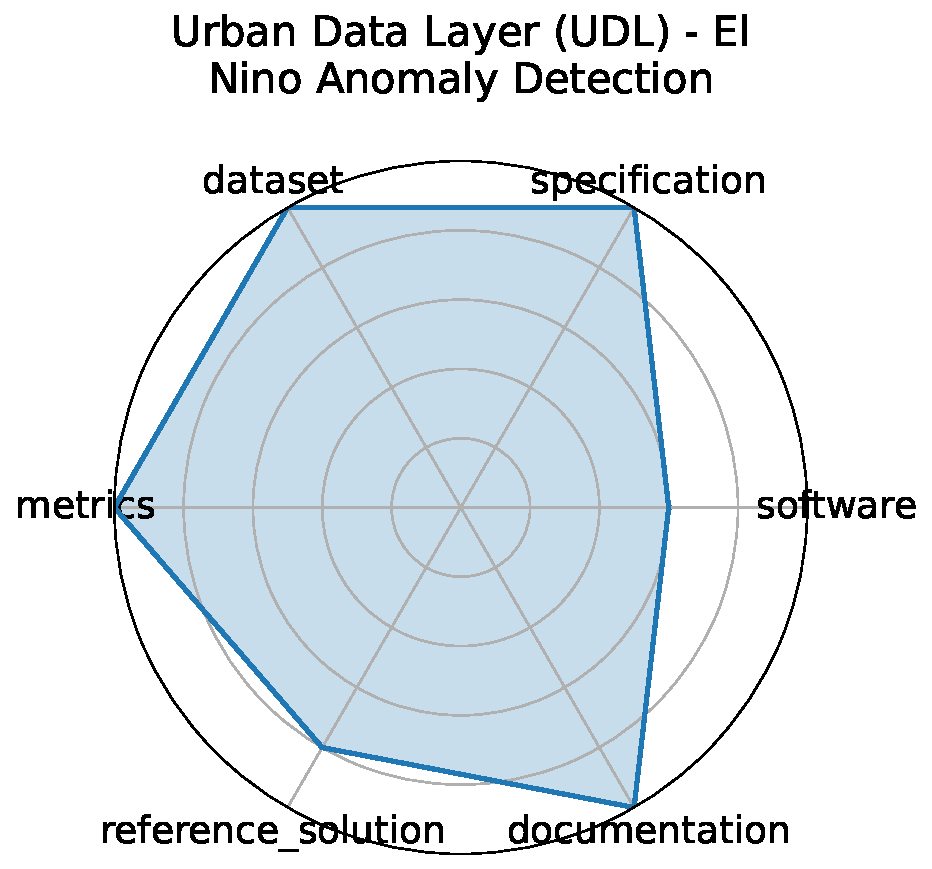
\includegraphics[width=0.15\textwidth]{urban_data_layer_udl_-_el_nino_anomaly_detection_radar.pdf} & Urban Data Layer (UDL) - El Nino Anomaly Detection & Climate \& Earth Science & Unified data pipeline for multi-modal urban science research & data pipeline, urban science, multi-modal, benchmark & Prediction, Classification & Anomaly Detection & Multi-modal urban inference, standardization & Task-specific accuracy or RMSE & Baseline regression/classification pipelines & \textbf{4.50} & \cite{neurips2024_0db7f135} \\ \hline
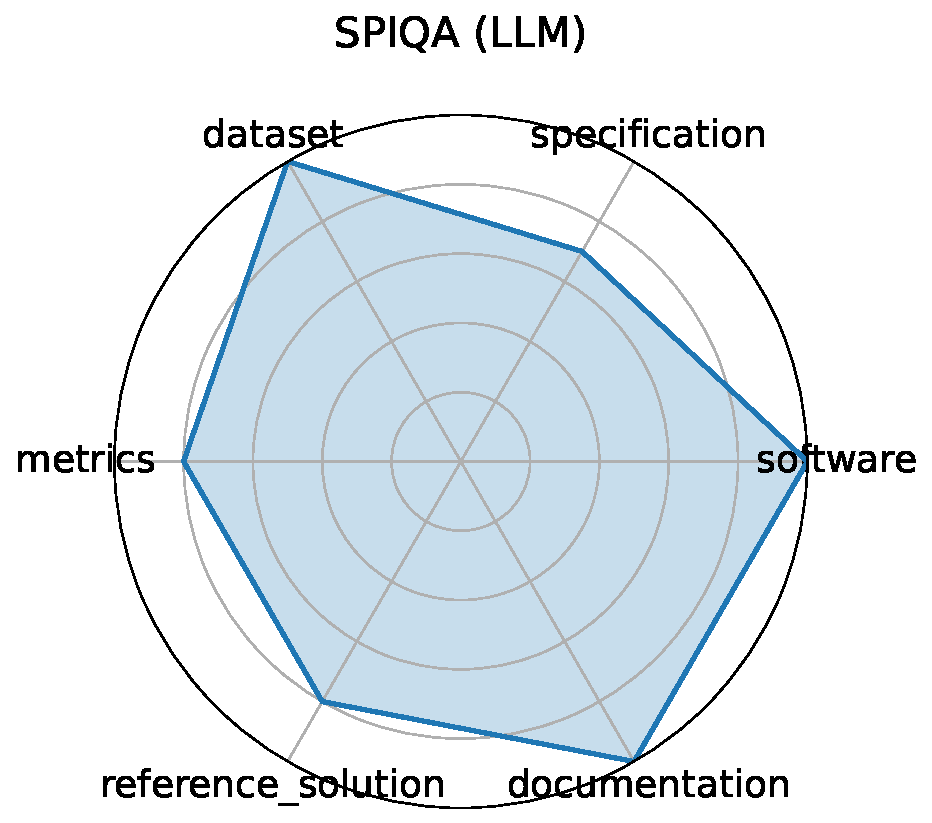
\includegraphics[width=0.15\textwidth]{spiqa_llm_radar.pdf} & SPIQA (LLM) & Computational Science \& AI & Evaluating LLMs on image-based scientific paper figure QA tasks (LLM Adapter performance) & multimodal QA, scientific figures, image+text, chain-of-thought prompting & Multimodal QA & Multimodal Reasoning & Visual reasoning, scientific figure understanding & Accuracy, F1 score & LLaVA, MiniGPT-4, Owl-LLM adapter variants & 4.42 & \cite{pramanick2025spiqadatasetmultimodalquestion} \\ \hline
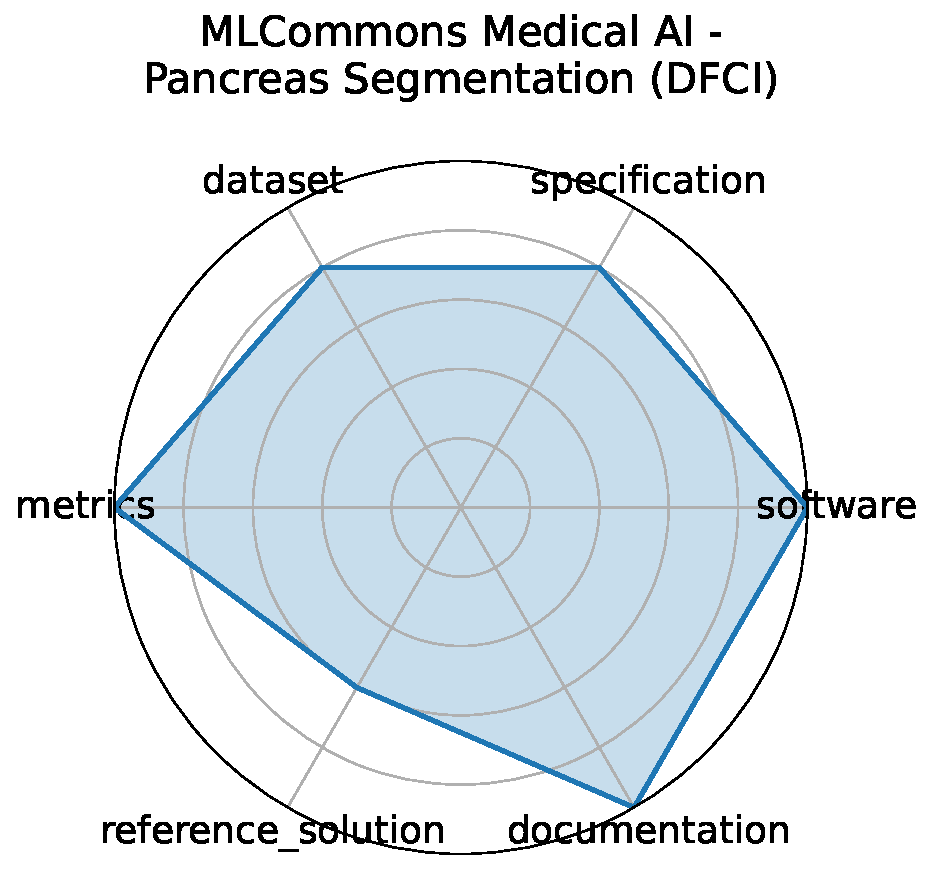
\includegraphics[width=0.15\textwidth]{mlcommons_medical_ai_-_pancreas_segmentation_dfci_radar.pdf} & MLCommons Medical AI - Pancreas Segmentation (DFCI) & Biology \& Medicine & Federated benchmarking and evaluation of medical AI models across diverse real-world clinical data & medical AI, federated evaluation, privacy-preserving, fairness, healthcare benchmarks & Federated evaluation, Model validation & Classification & Clinical accuracy, fairness, generalizability, privacy compliance & ROC AUC, Accuracy, Fairness metrics & MedPerf-validated CNNs, GaNDLF workflows & 4.33 & \cite{karargyris2023federated} \\ \hline
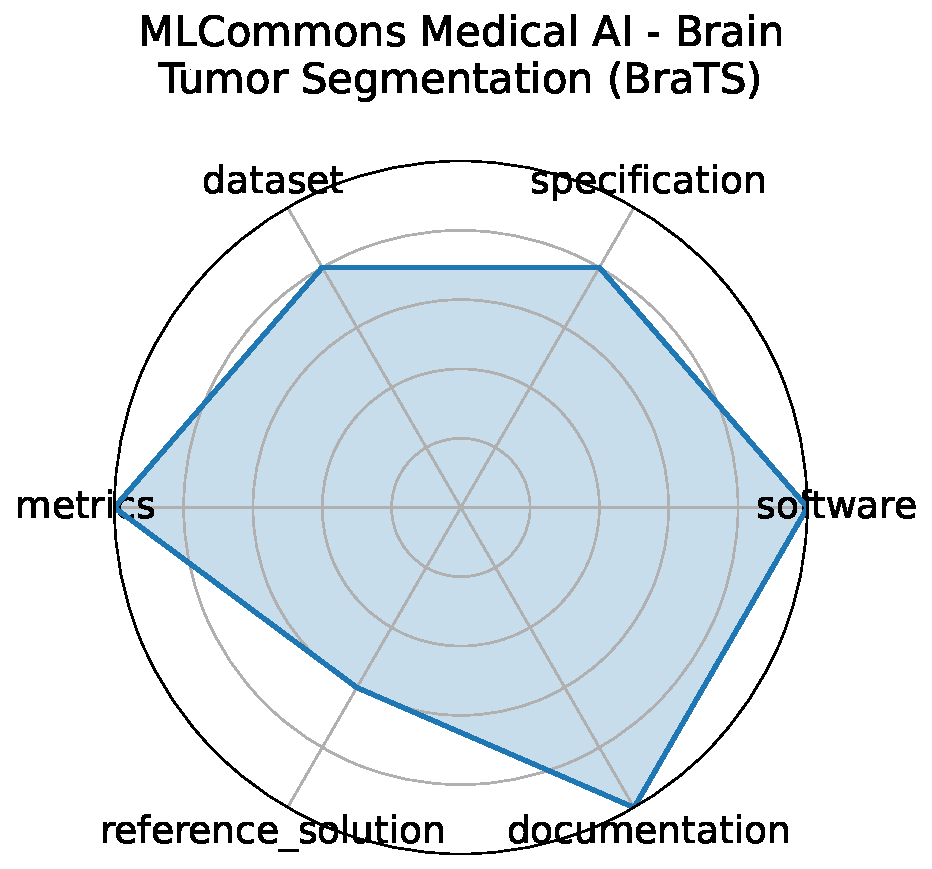
\includegraphics[width=0.15\textwidth]{mlcommons_medical_ai_-_brain_tumor_segmentation_brats_radar.pdf} & MLCommons Medical AI - Brain Tumor Segmentation (BraTS) & Biology \& Medicine & Federated benchmarking and evaluation of medical AI models across diverse real-world clinical data & medical AI, federated evaluation, privacy-preserving, fairness, healthcare benchmarks & Federated evaluation, Model validation & Classification & Clinical accuracy, fairness, generalizability, privacy compliance & ROC AUC, Accuracy, Fairness metrics & MedPerf-validated CNNs, GaNDLF workflows & 4.33 & \cite{karargyris2023federated} \\ \hline
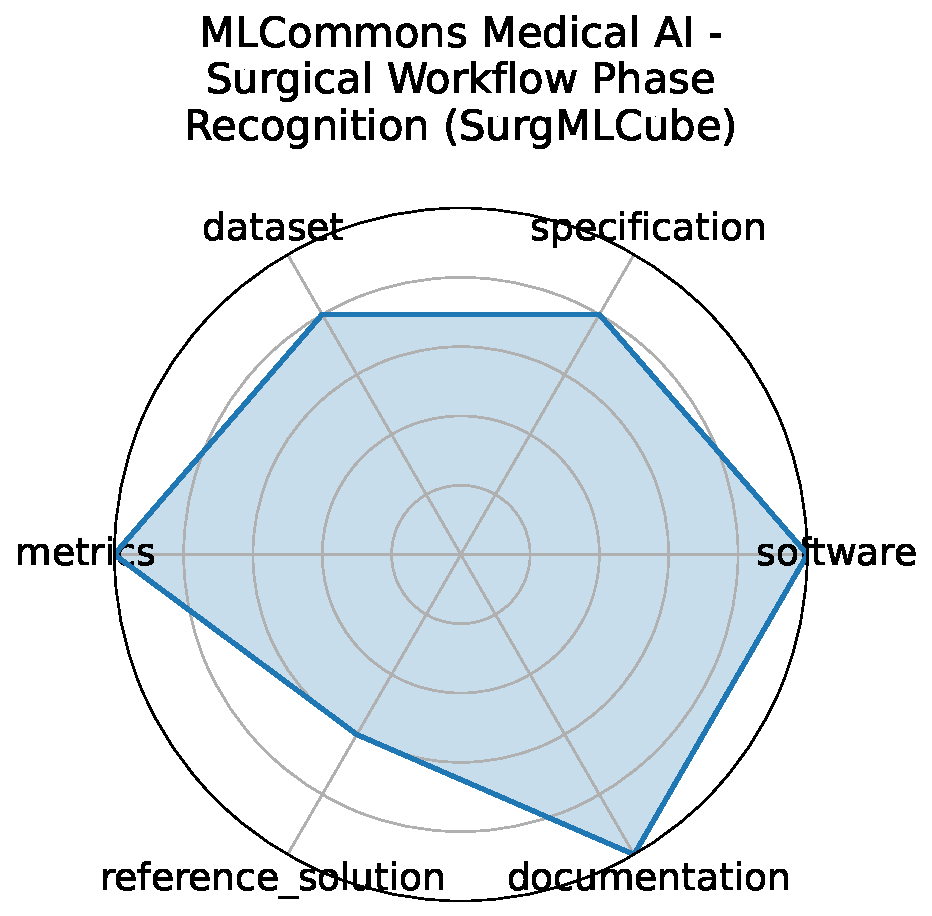
\includegraphics[width=0.15\textwidth]{mlcommons_medical_ai_-__surgical_workflow_phase_recognition_surgmlcube_radar.pdf} & MLCommons Medical AI -  Surgical Workflow Phase Recognition (SurgMLCube) & Biology \& Medicine & Federated benchmarking and evaluation of medical AI models across diverse real-world clinical data & medical AI, federated evaluation, privacy-preserving, fairness, healthcare benchmarks & Federated evaluation, Model validation & Classification & Clinical accuracy, fairness, generalizability, privacy compliance & ROC AUC, Accuracy, Fairness metrics & MedPerf-validated CNNs, GaNDLF workflows & 4.33 & \cite{karargyris2023federated} \\ \hline
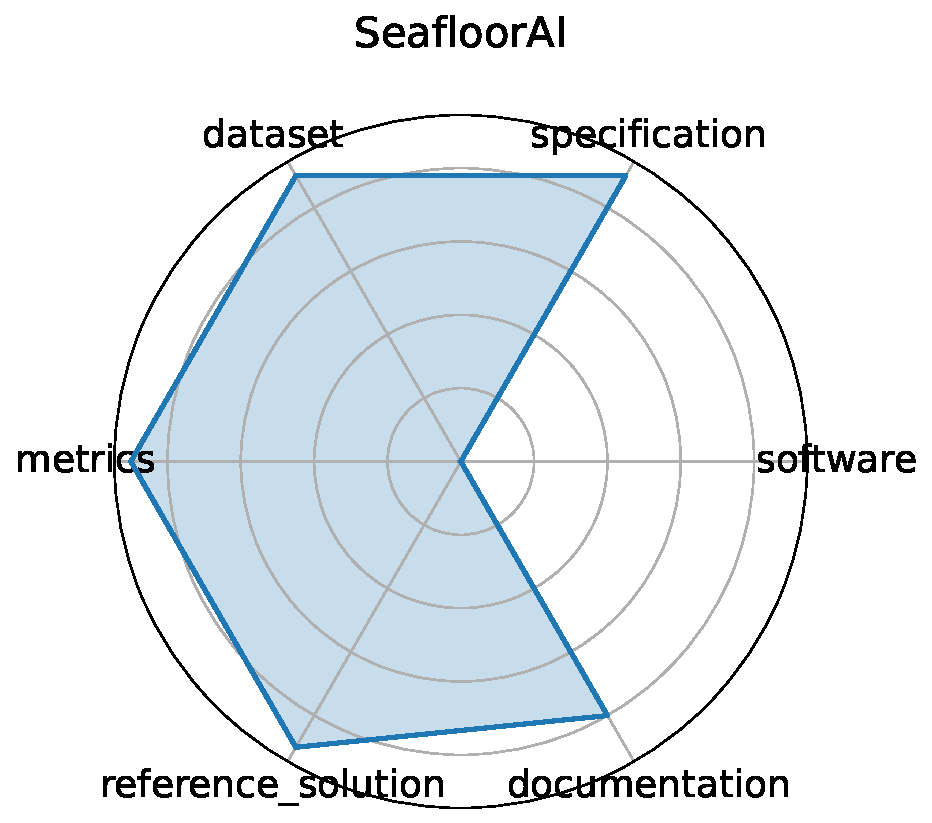
\includegraphics[width=0.15\textwidth]{seafloorai_radar.pdf} & SeafloorAI & Climate \& Earth Science & Large-scale vision-language dataset for seafloor mapping and geological classification & sonar imagery, vision-language, seafloor mapping, segmentation, QA & Image segmentation, Vision-language QA & Classification & Geospatial understanding, multimodal reasoning & Segmentation pixel accuracy, QA accuracy & SegFormer, ViLT-style multimodal models & 4.33 & \cite{nguyen2024seafloor} \\ \hline
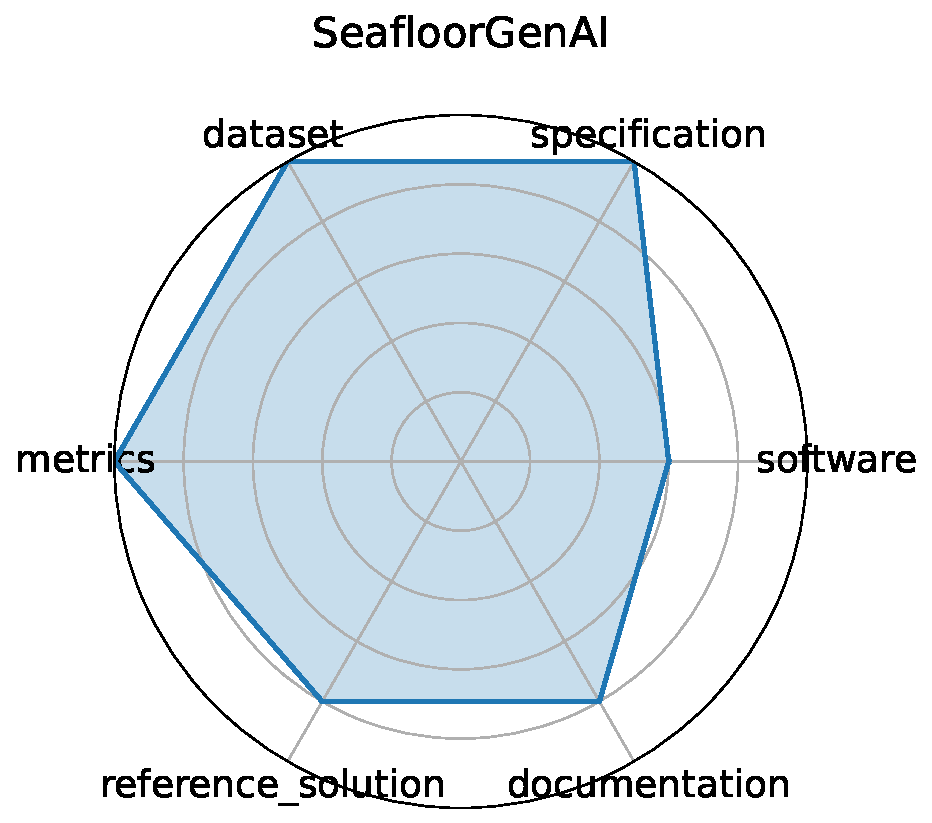
\includegraphics[width=0.15\textwidth]{seafloorgenai_radar.pdf} & SeafloorGenAI & Climate \& Earth Science & Large-scale vision-language dataset for seafloor mapping and geological classification & sonar imagery, vision-language, seafloor mapping, segmentation, QA & Image segmentation, Vision-language QA & Reasoning \& Generalization & Geospatial understanding, multimodal reasoning & Segmentation pixel accuracy, QA accuracy & SegFormer, ViLT-style multimodal models & 4.33 & \cite{nguyen2024seafloor} \\ \hline
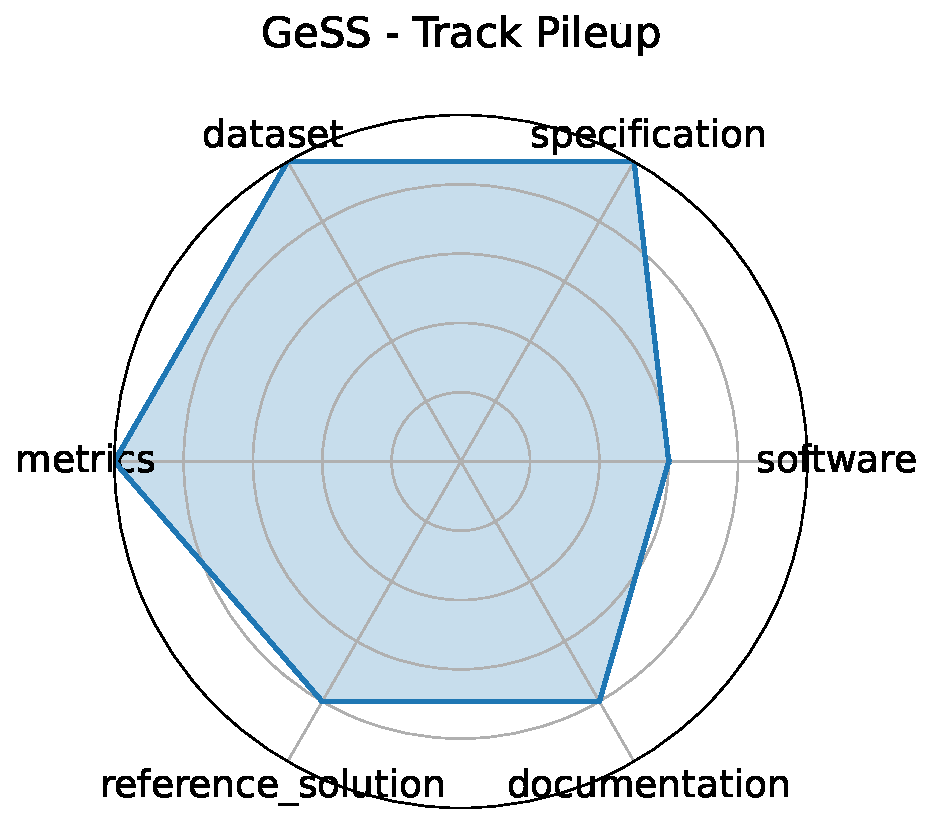
\includegraphics[width=0.15\textwidth]{gess_-_track_pileup_radar.pdf} & GeSS - Track Pileup & High Energy Physics & Benchmark suite evaluating geometric deep learning models under real-world distribution shifts & geometric deep learning, distribution shift, OOD robustness, scientific applications & Classification & Classification & OOD performance in scientific settings & Accuracy, RMSE, OOD robustness delta & GCN, EGNN, DimeNet++ & 4.33 & \cite{neurips2024_a8063075} \\ \hline
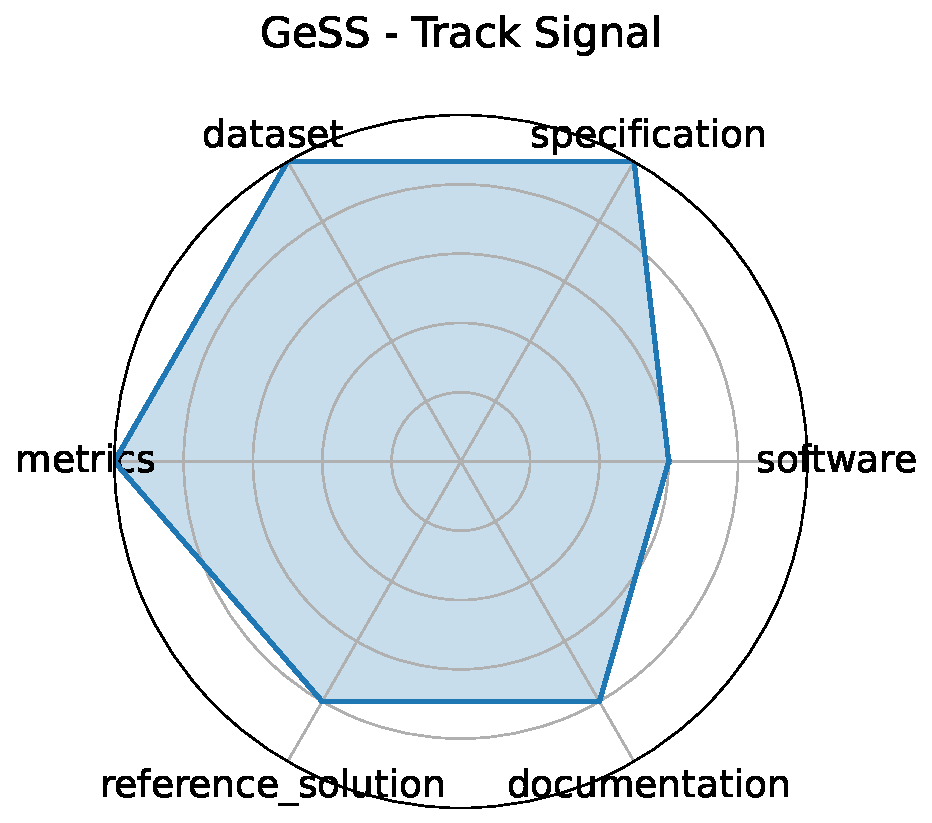
\includegraphics[width=0.15\textwidth]{gess_-_track_signal_radar.pdf} & GeSS - Track Signal & High Energy Physics & Benchmark suite evaluating geometric deep learning models under real-world distribution shifts & geometric deep learning, distribution shift, OOD robustness, scientific applications & Classification & Classification & OOD performance in scientific settings & Accuracy, RMSE, OOD robustness delta & GCN, EGNN, DimeNet++ & 4.33 & \cite{neurips2024_a8063075} \\ \hline
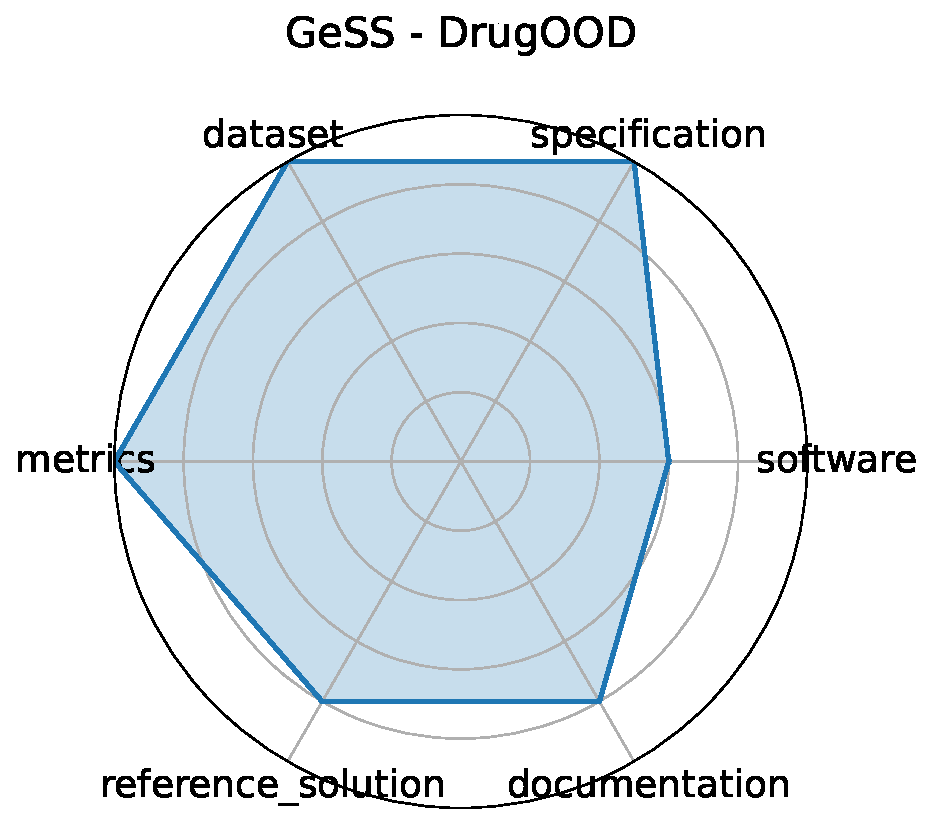
\includegraphics[width=0.15\textwidth]{gess_-_drugood_radar.pdf} & GeSS - DrugOOD & Biology \& Medicine & Benchmark suite evaluating geometric deep learning models under real-world distribution shifts & geometric deep learning, distribution shift, OOD robustness, scientific applications & Classification & Classification & OOD performance in scientific settings & Accuracy, RMSE, OOD robustness delta & GCN, EGNN, DimeNet++ & 4.33 & \cite{neurips2024_a8063075} \\ \hline
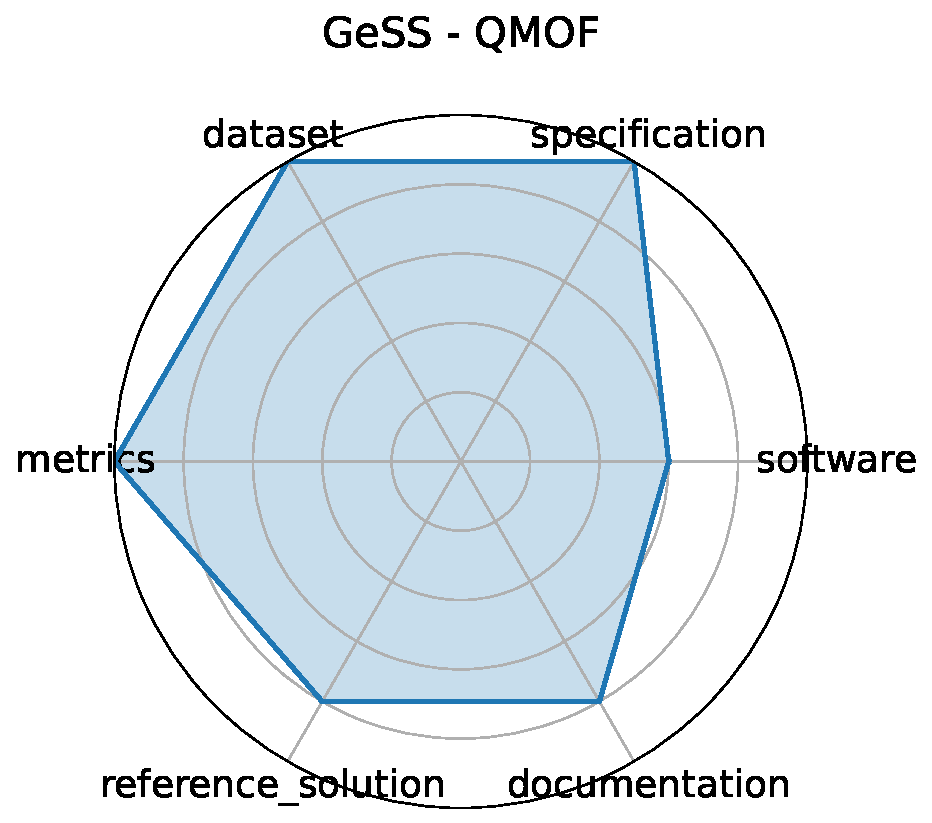
\includegraphics[width=0.15\textwidth]{gess_-_qmof_radar.pdf} & GeSS - QMOF & Materials Science & Benchmark suite evaluating geometric deep learning models under real-world distribution shifts & geometric deep learning, distribution shift, OOD robustness, scientific applications & Classification, Regression & Regression & OOD performance in scientific settings & Accuracy, RMSE, OOD robustness delta & GCN, EGNN, DimeNet++ & 4.33 & \cite{neurips2024_a8063075} \\ \hline
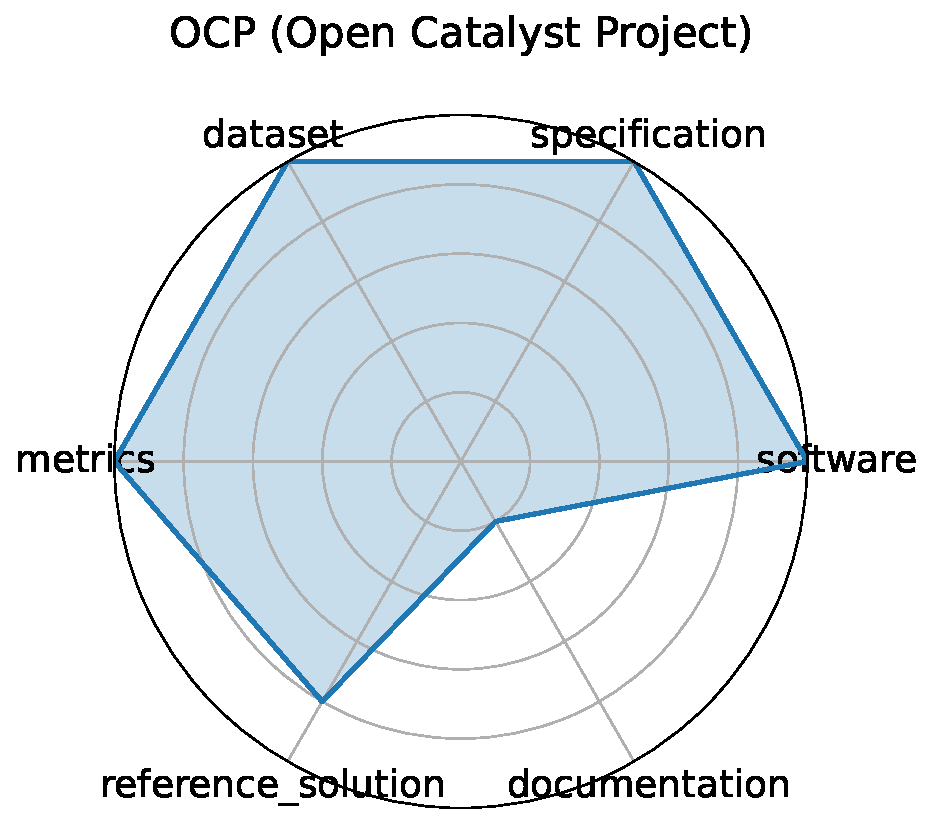
\includegraphics[width=0.15\textwidth]{ocp_open_catalyst_project_radar.pdf} & OCP (Open Catalyst Project) & Chemistry, Materials Science & Catalyst adsorption energy prediction & DFT relaxations, adsorption energy, graph neural networks & Energy prediction, Force prediction & Regression & Prediction of adsorption energies and forces & MAE (energy), MAE (force) & CGCNN, SchNet, DimeNet++, GemNet-OC & 4.17 & \cite{chanussot2021oc20,tran2023oc22,doi:10.1021/acscatal.0c04525,tran2023b} \\ \hline
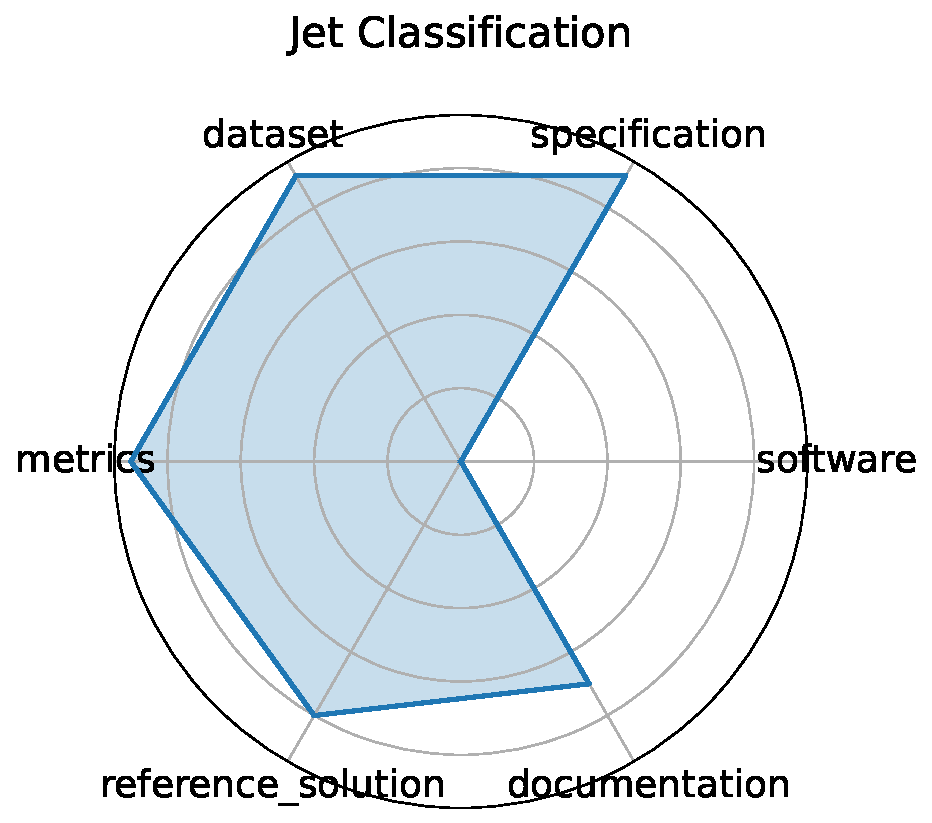
\includegraphics[width=0.15\textwidth]{jet_classification_radar.pdf} & Jet Classification & High Energy Physics & Real-time classification of particle jets using HL-LHC simulation features & classification, real-time ML, jet tagging, QKeras & Classification & Classification & Real-time inference, model compression performance & Accuracy, AUC & Keras DNN, QKeras quantized DNN & 4.17 & \cite{duarte2022fastml} \\ \hline
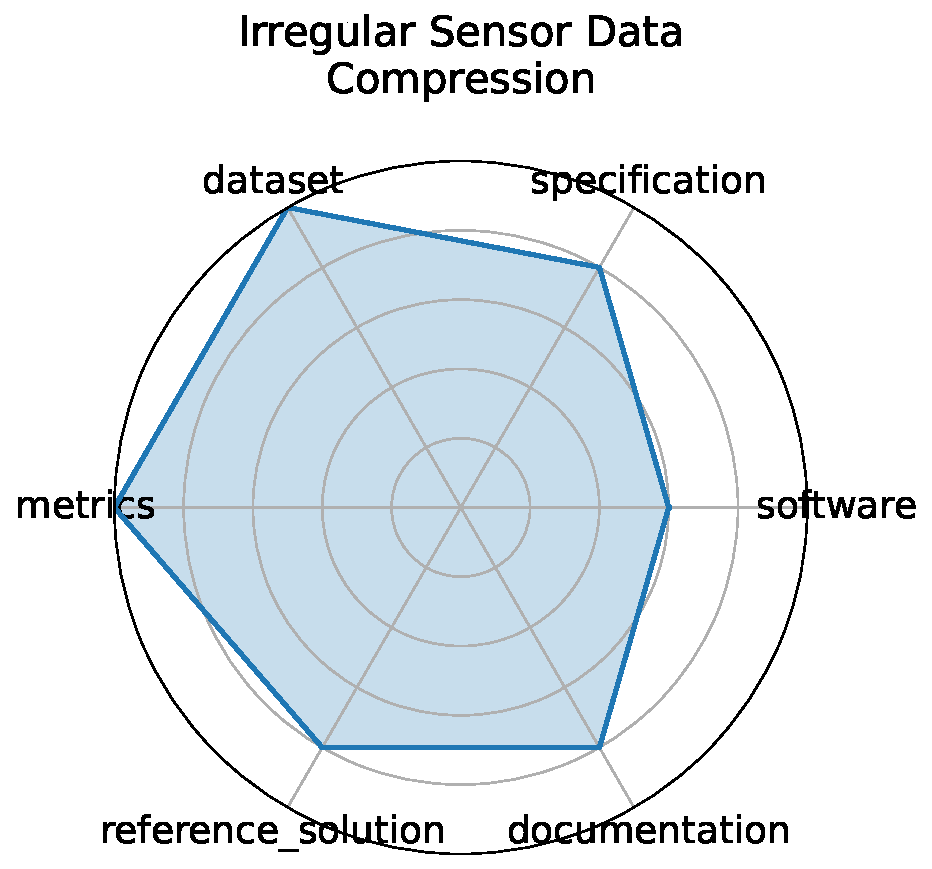
\includegraphics[width=0.15\textwidth]{irregular_sensor_data_compression_radar.pdf} & Irregular Sensor Data Compression & High Energy Physics & Real-time compression of sparse sensor data with autoencoders & compression, autoencoder, sparse data, irregular sampling & Compression & Generative & Reconstruction quality, compression efficiency & MSE, Compression ratio & Autoencoder, Quantized autoencoder & 4.17 & \cite{duarte2022fastmlsciencebenchmarksaccelerating2} \\ \hline
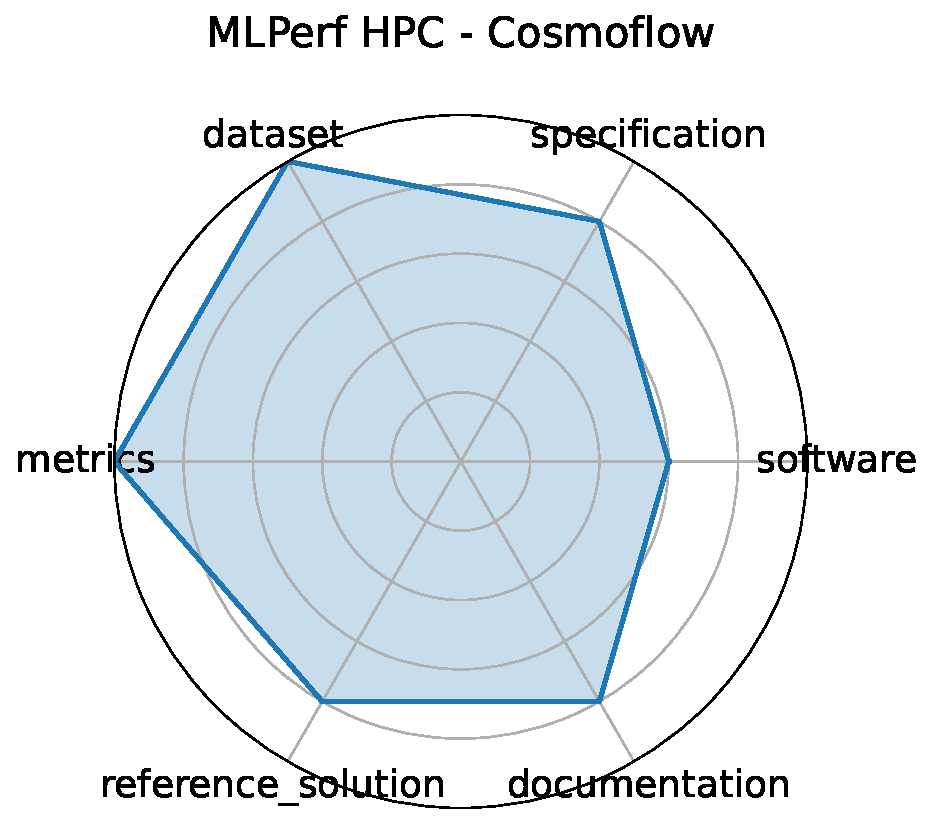
\includegraphics[width=0.15\textwidth]{mlperf_hpc_-_cosmoflow_radar.pdf} & MLPerf HPC - Cosmoflow & High Energy Physics & Scientific ML training and inference on HPC systems & HPC, training, inference, scientific ML & Training, Inference & Regression & Scaling efficiency, training time, model accuracy on HPC & Training time, Accuracy, GPU utilization & CosmoFlow, DeepCAM, OpenCatalyst & 4.17 & \cite{farrell2021mlperfhpcholisticbenchmark} \\ \hline
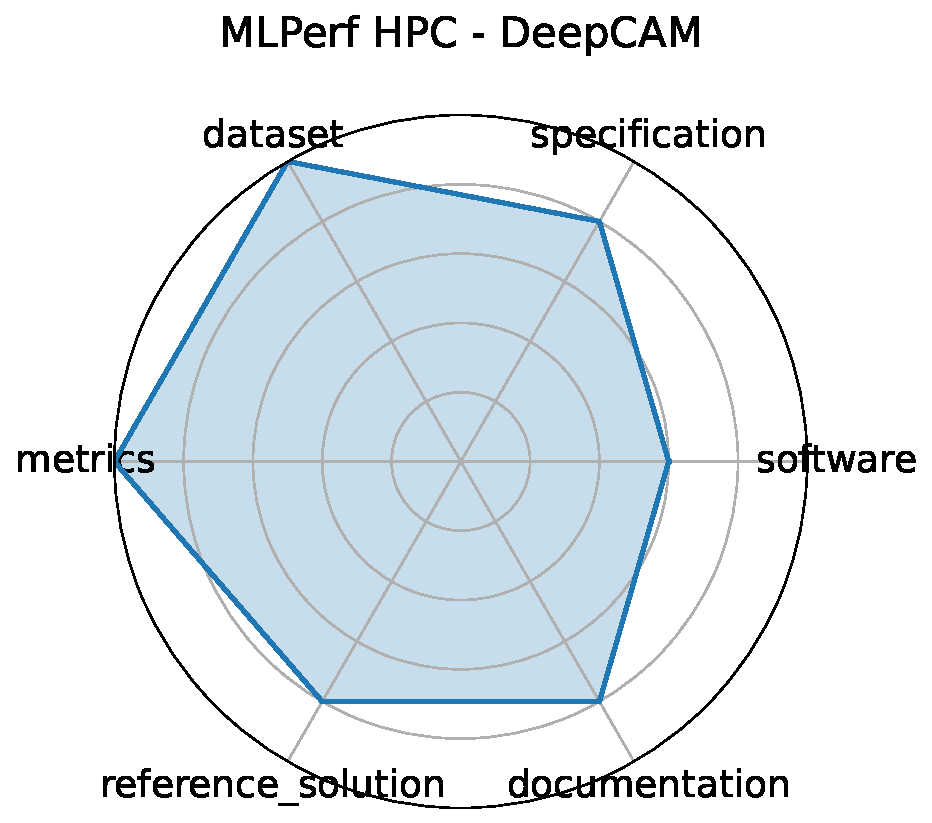
\includegraphics[width=0.15\textwidth]{mlperf_hpc_-_deepcam_radar.pdf} & MLPerf HPC - DeepCAM & Climate \& Earth Science & Scientific ML training and inference on HPC systems & HPC, training, inference, scientific ML & Training, Inference & Classification & Scaling efficiency, training time, model accuracy on HPC & Training time, Accuracy, GPU utilization & DeepCAM & 4.17 & \cite{farrell2021mlperfhpcholisticbenchmark} \\ \hline
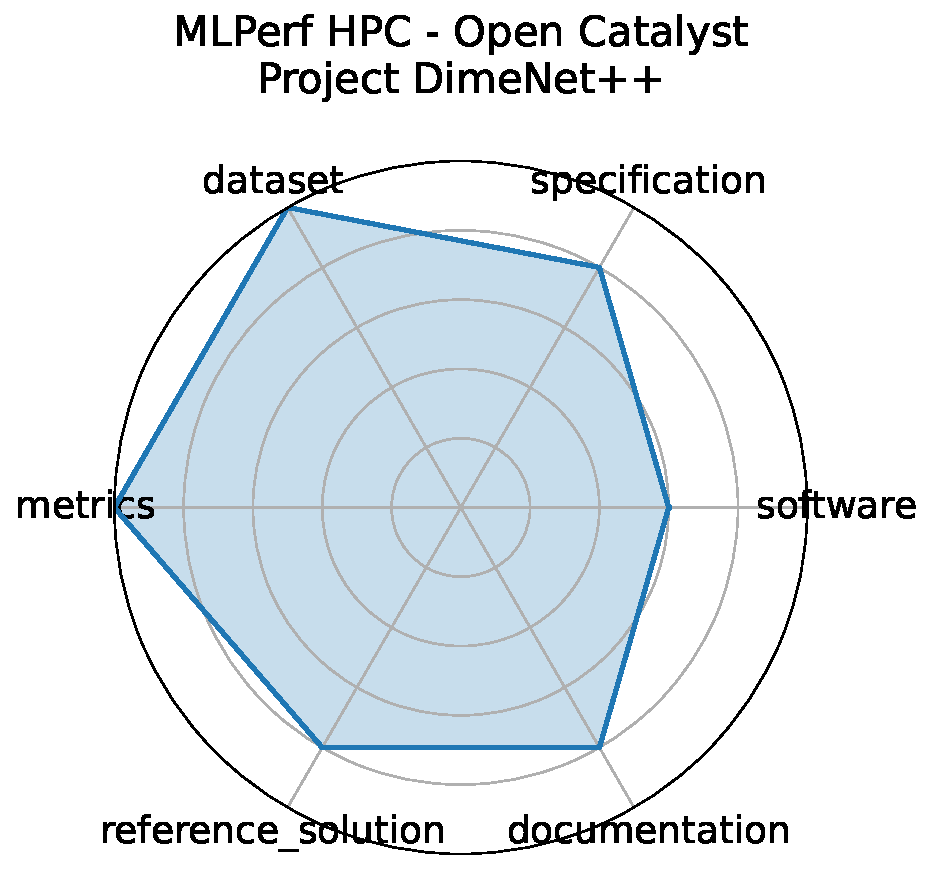
\includegraphics[width=0.15\textwidth]{mlperf_hpc_-_open_catalyst_project_dimenet__radar.pdf} & MLPerf HPC - Open Catalyst Project DimeNet++  & Chemistry & Scientific ML training and inference on HPC systems & HPC, training, inference, scientific ML & Training, Inference & Regression & Scaling efficiency, training time, model accuracy on HPC & Training time, Accuracy, GPU utilization & DeepCAM & 4.17 & \cite{farrell2021mlperfhpcholisticbenchmark} \\ \hline
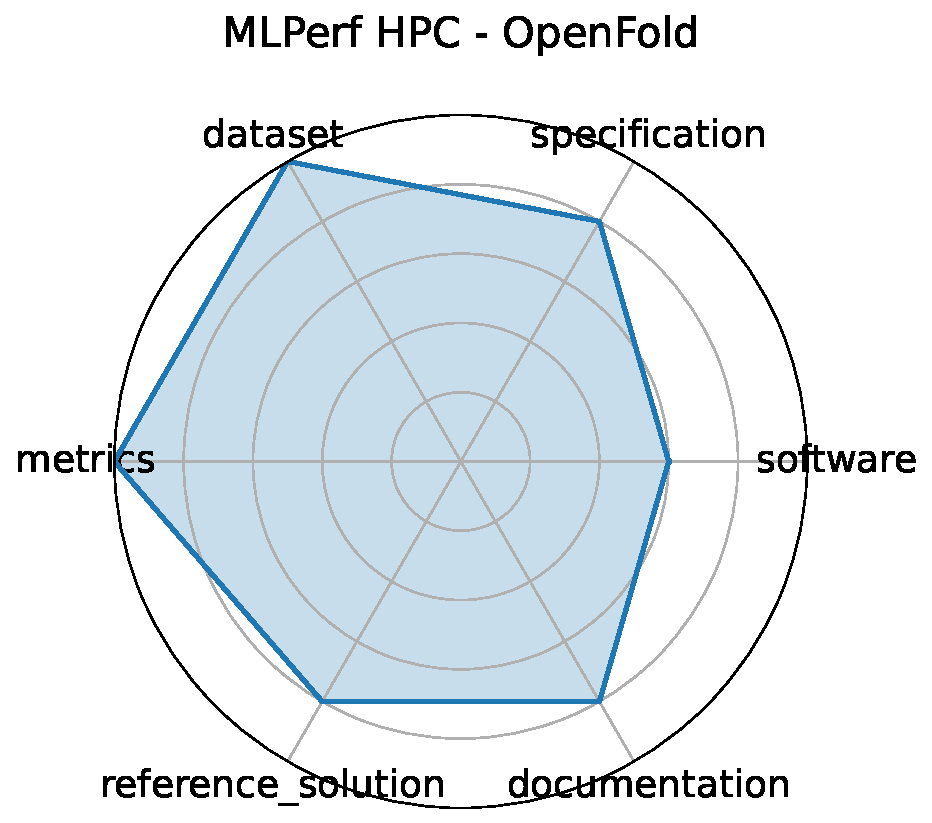
\includegraphics[width=0.15\textwidth]{mlperf_hpc_-_openfold_radar.pdf} & MLPerf HPC - OpenFold & Biology \& Medicine & Scientific ML training and inference on HPC systems & HPC, training, inference, scientific ML & Training, Inference & Sequence Prediction/Forecasting & Scaling efficiency, training time, model accuracy on HPC & Training time, Accuracy, GPU utilization & DeepCAM & 4.17 & \cite{farrell2021mlperfhpcholisticbenchmark} \\ \hline
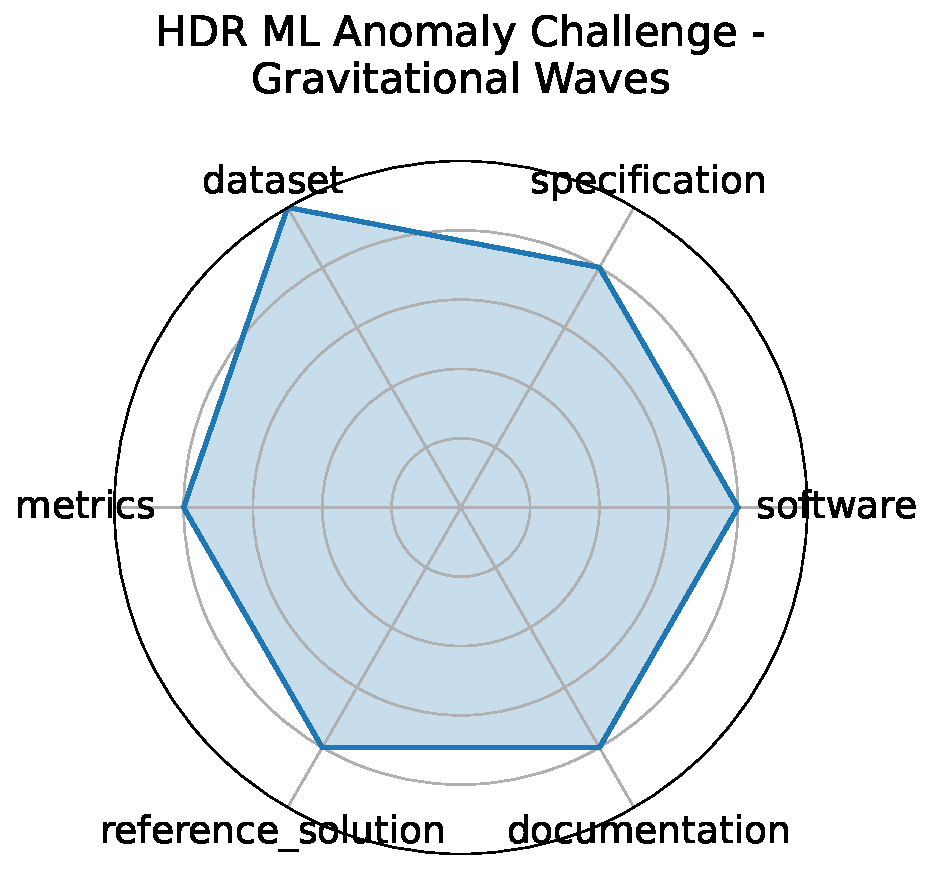
\includegraphics[width=0.15\textwidth]{hdr_ml_anomaly_challenge_-_gravitational_waves_radar.pdf} & HDR ML Anomaly Challenge - Gravitational Waves & High Energy Physics & Detecting anomalous gravitational-wave signals from LIGO/Virgo datasets & anomaly detection, gravitational waves, astrophysics, time-series & Anomaly Detection & Anomaly Detection & Novel event detection in physical signals & ROC-AUC, Precision/Recall & Deep latent CNNs, Autoencoders & 4.17 & \cite{campolongo2025buildingmachinelearningchallenges} \\ \hline
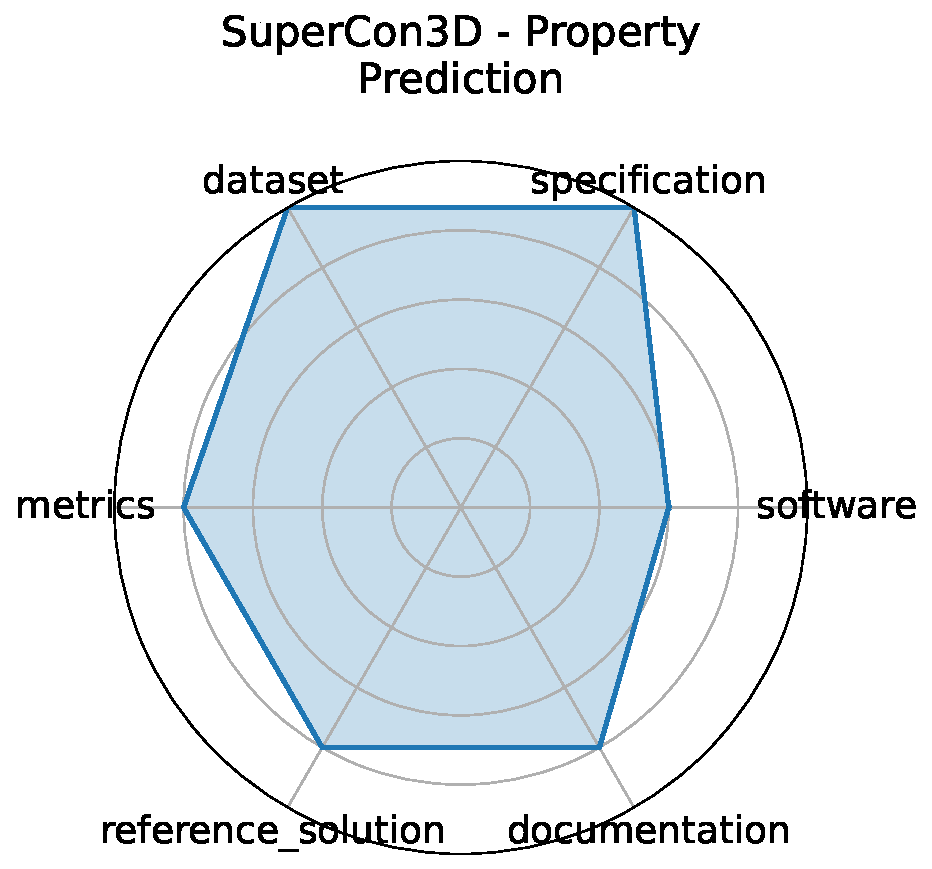
\includegraphics[width=0.15\textwidth]{supercond_-_property_prediction_radar.pdf} & SuperCon3D - Property Prediction & Materials Science & Dataset and models for predicting and generating high-Tc superconductors using 3D crystal structures & superconductivity, crystal structures, equivariant GNN, generative models & Regression (Tc prediction), Generative modeling & Regression & Structure-to-property prediction, structure generation & MAE (Tc), Validity of generated structures & SODNet, DiffCSP-SC & 4.17 & \cite{neurips2024_c4e3b55e} \\ \hline
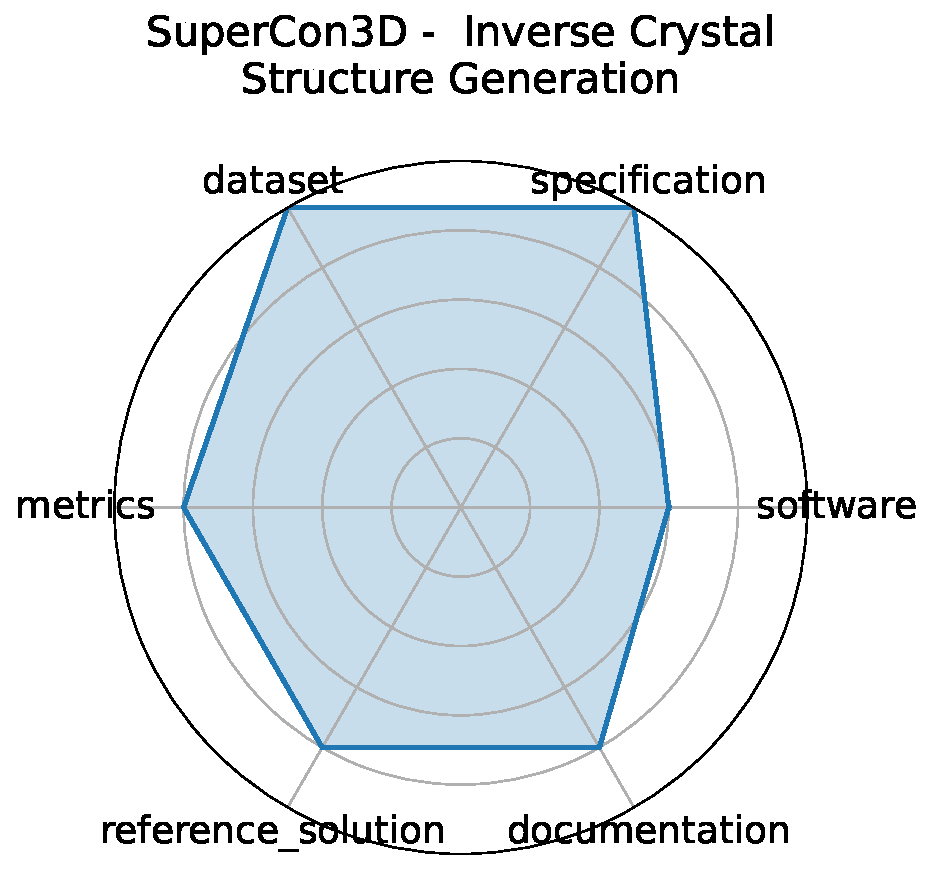
\includegraphics[width=0.15\textwidth]{supercond_-__inverse_crystal_structure_generation_radar.pdf} & SuperCon3D -  Inverse Crystal Structure Generation & Materials Science & Dataset and models for predicting and generating high-Tc superconductors using 3D crystal structures & superconductivity, crystal structures, equivariant GNN, generative models & Regression (Tc prediction), Generative modeling & Generative & Structure-to-property prediction, structure generation & MAE (Tc), Validity of generated structures & SODNet, DiffCSP-SC & 4.17 & \cite{neurips2024_c4e3b55e} \\ \hline
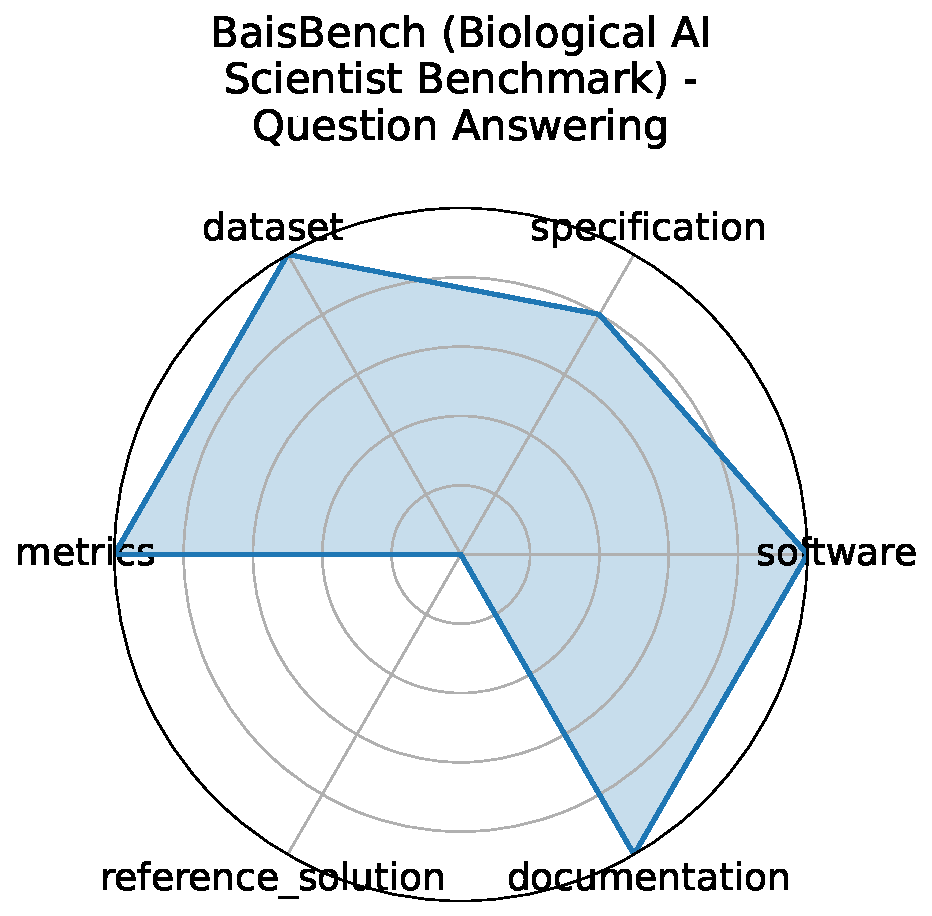
\includegraphics[width=0.15\textwidth]{baisbench_biological_ai_scientist_benchmark_-_question_answering_radar.pdf} & BaisBench (Biological AI Scientist Benchmark) - Question Answering & Biology \& Medicine & Omics-driven AI research tasks & single-cell annotation, biological QA, autonomous discovery & Cell type annotation, Multiple choice & Reasoning \& Generalization & Autonomous biological research capabilities & Annotation accuracy, QA accuracy & LLM-based AI scientist agents & 4.00 & \cite{luo2025benchmarkingaiscientistsomics} \\ \hline
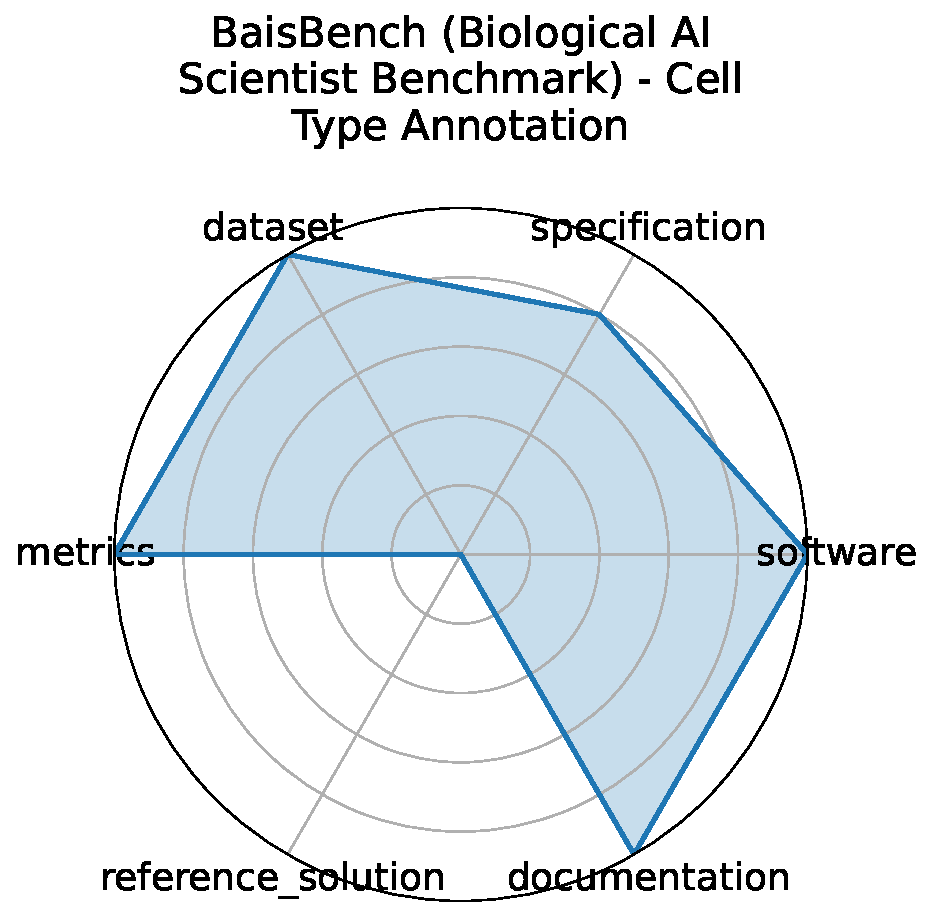
\includegraphics[width=0.15\textwidth]{baisbench_biological_ai_scientist_benchmark_-_cell_type_annotation_radar.pdf} & BaisBench (Biological AI Scientist Benchmark) - Cell Type Annotation & Biology \& Medicine & Omics-driven AI research tasks & single-cell annotation, biological QA, autonomous discovery & Cell type annotation, Multiple choice & Classification & Autonomous biological research capabilities & Annotation accuracy, QA accuracy & LLM-based AI scientist agents & 4.00 & \cite{luo2025benchmarkingaiscientistsomics} \\ \hline
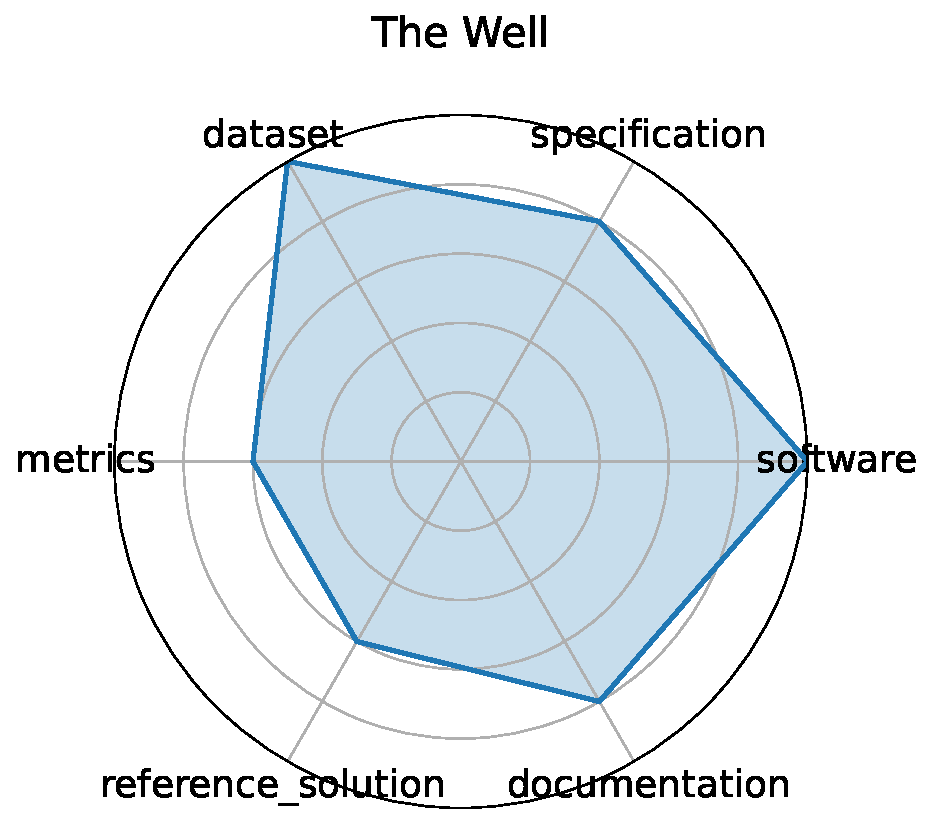
\includegraphics[width=0.15\textwidth]{the_well_radar.pdf} & The Well & Biology \& Medicine, Computational Science \& AI, High Energy Physics & Foundation model + surrogate dataset spanning 16 physical simulation domains & surrogate modeling, foundation model, physics simulations, spatiotemporal dynamics & Supervised Learning & Sequence Prediction/Forecasting & Surrogate modeling, physics-based prediction & Dataset size, Domain breadth & FNO baselines, U-Net baselines & 4.00 & \cite{neurips2024_4f9a5acd} \\ \hline
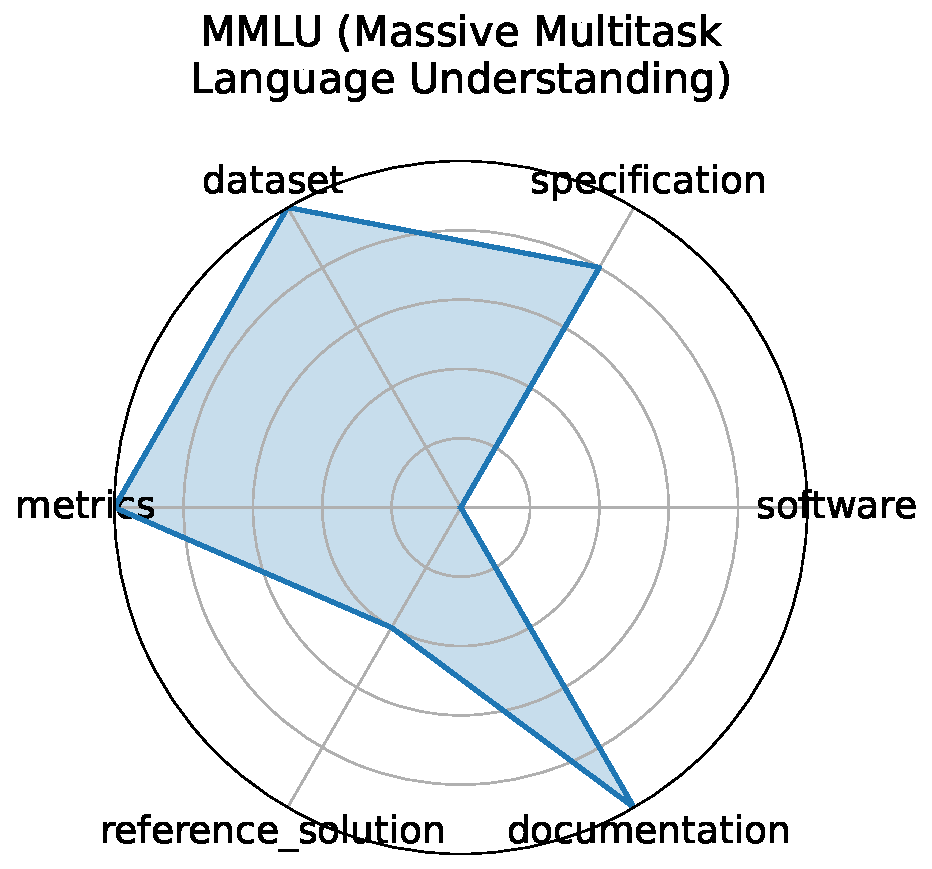
\includegraphics[width=0.15\textwidth]{mmlu_massive_multitask_language_understanding_radar.pdf} & MMLU (Massive Multitask Language Understanding) & Computational Science \& AI & Academic knowledge and reasoning across 57 subjects & multitask, multiple-choice, zero-shot, few-shot, knowledge probing & Multiple choice & Reasoning \& Generalization & General reasoning, subject-matter understanding & Accuracy & GPT-4o, Gemini 1.5 Pro, o1, DeepSeek-R1 & 3.83 & \cite{hendrycks2021measuring} \\ \hline
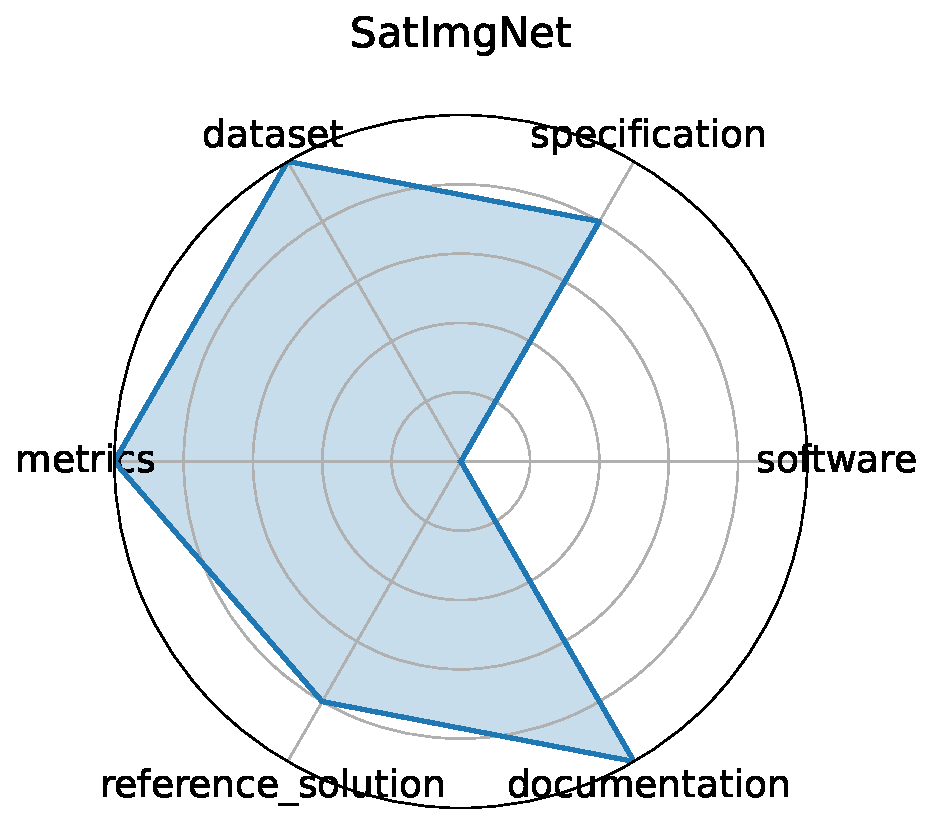
\includegraphics[width=0.15\textwidth]{satimgnet_radar.pdf} & SatImgNet & Climate \& Earth Science & Satellite imagery classification & land-use, zero-shot, multi-task & Image classification & Multimodal Reasoning & Zero-shot land-use classification & Accuracy & CLIP, BLIP, ALBEF & 3.83 & \cite{roberts2023satin} \\ \hline
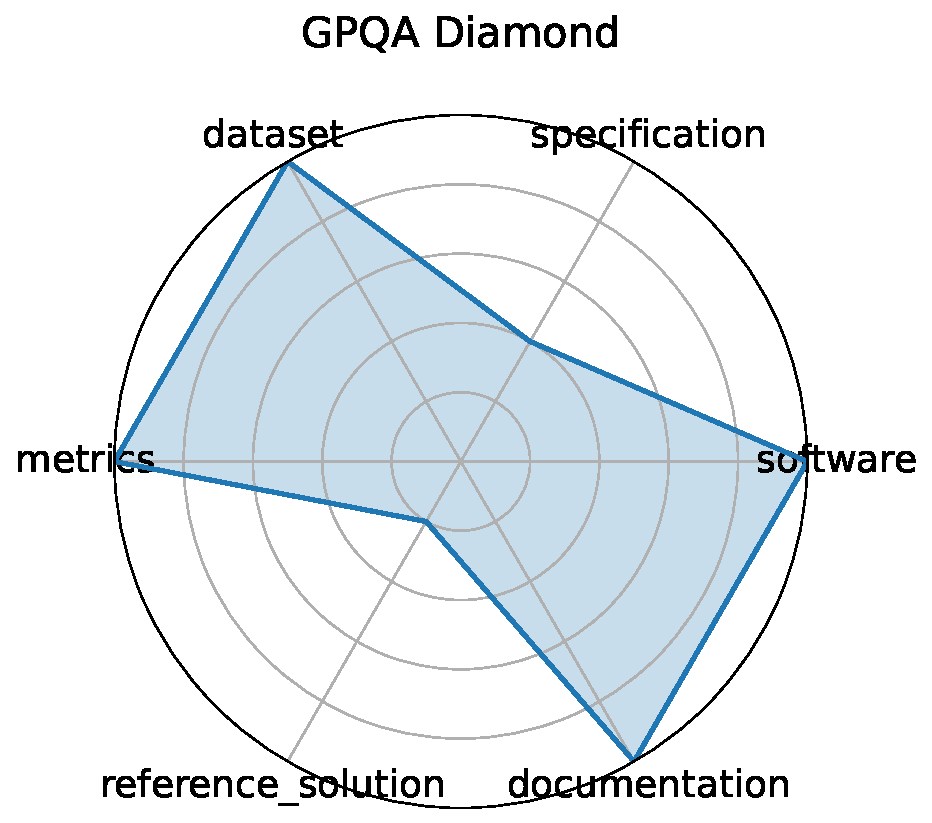
\includegraphics[width=0.15\textwidth]{gpqa_diamond_radar.pdf} & GPQA Diamond & Biology \& Medicine, Chemistry, High Energy Physics & Graduate-level scientific reasoning & Google-proof, graduate-level, science QA, chemistry, physics & Multiple choice, Multi-step QA & Reasoning \& Generalization & Scientific reasoning, deep knowledge & Accuracy & o1, DeepSeek-R1 & 3.83 & \cite{rein2023gpqagraduatelevelgoogleproofqa} \\ \hline
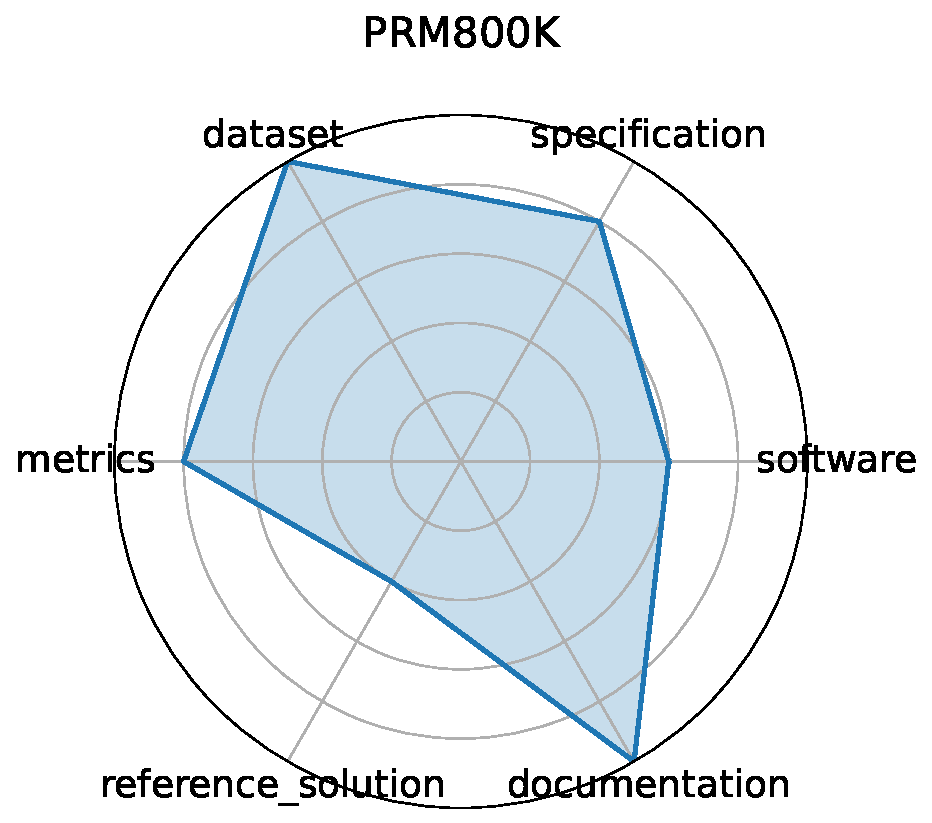
\includegraphics[width=0.15\textwidth]{prmk_radar.pdf} & PRM800K & Mathematics & Math reasoning generalization & calculus, algebra, number theory, geometry & Problem solving & Reasoning \& Generalization & Math reasoning and generalization & Accuracy & GPT-4 & 3.83 & \cite{lightman2023lets} \\ \hline
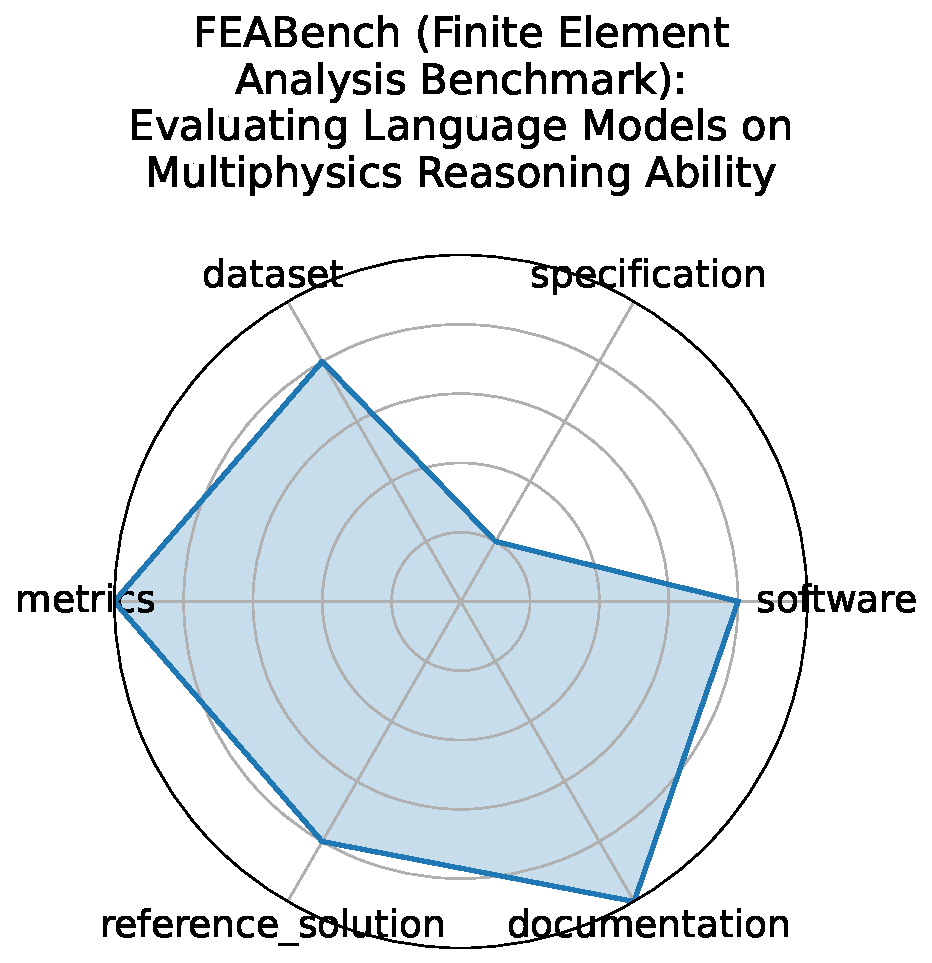
\includegraphics[width=0.15\textwidth]{feabench_finite_element_analysis_benchmark_evaluating_language_models_on_multiphysics_reasoning_ability_radar.pdf} & FEABench (Finite Element Analysis Benchmark): Evaluating Language Models on Multiphysics Reasoning Ability & Mathematics & FEA simulation accuracy and performance & finite element, simulation, PDE & Simulation, Performance evaluation & Reasoning \& Generalization & Numerical simulation accuracy and efficiency & Solve time, Error norm & FEniCS, deal.II & 3.83 & \cite{mudur2025feabenchevaluatinglanguagemodels} \\ \hline
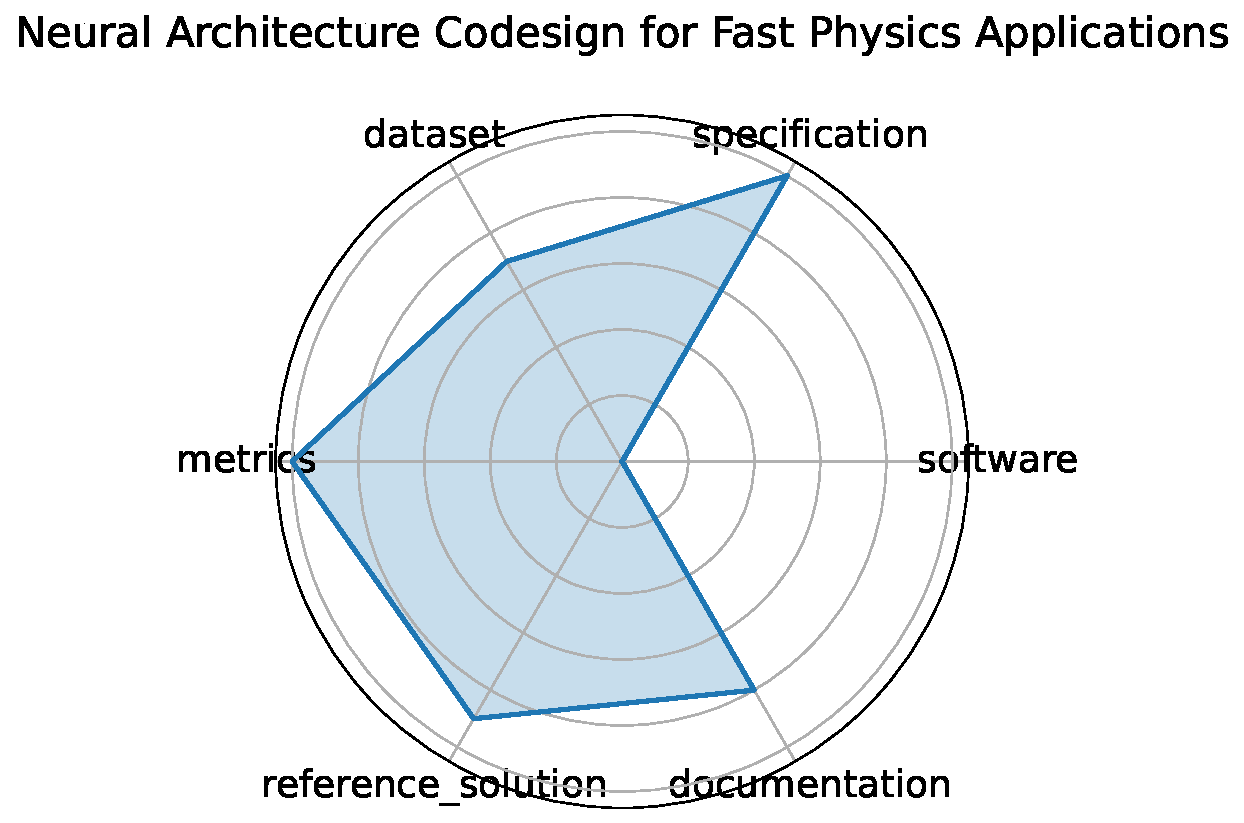
\includegraphics[width=0.15\textwidth]{neural_architecture_codesign_for_fast_physics_applications_radar.pdf} & Neural Architecture Codesign for Fast Physics Applications & High Energy Physics & Automated neural architecture search and hardware-efficient model codesign for fast physics applications & neural architecture search, FPGA deployment, quantization, pruning, hls4ml & Classification, Peak finding & Classification & Hardware-aware model optimization; low-latency inference & Accuracy, Latency, Resource utilization & NAC-based BraggNN, NAC-optimized Deep Sets (jet) & 3.83 & \cite{weitz2025neuralarchitecturecodesignfast} \\ \hline
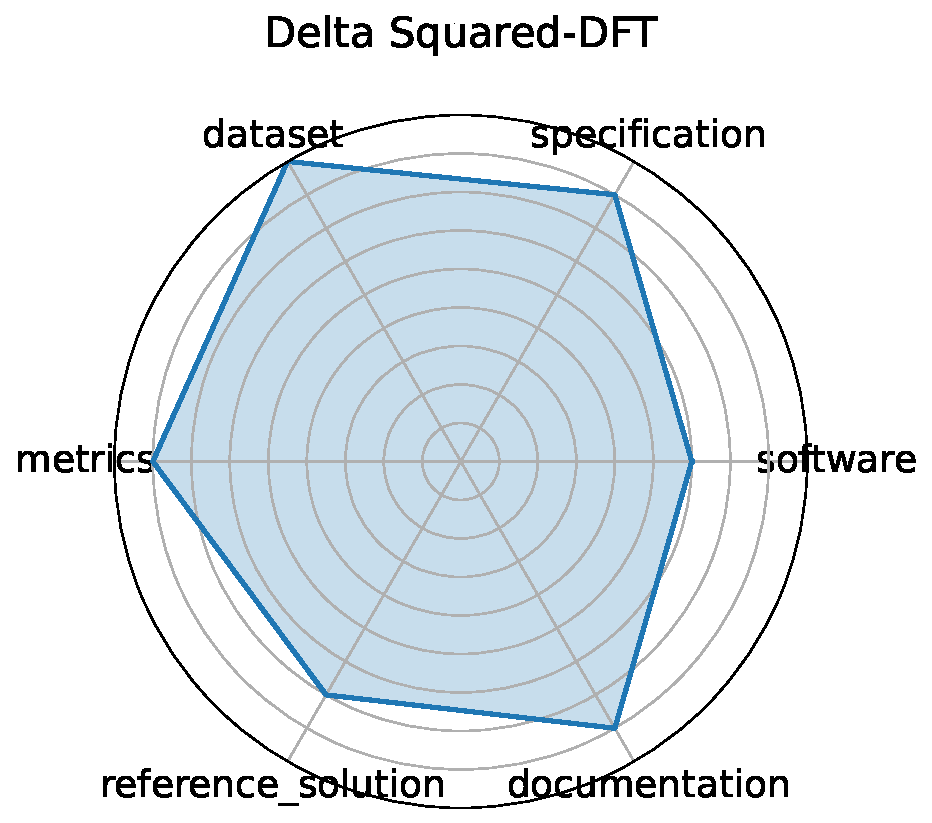
\includegraphics[width=0.15\textwidth]{delta_squared-dft_radar.pdf} & Delta Squared-DFT & Chemistry, Materials Science & Benchmarking machine-learning corrections to DFT using Delta Squared-trained models for reaction energies & density functional theory, Delta Squared-ML correction, reaction energetics, quantum chemistry & Regression & Regression & High-accuracy energy prediction, DFT correction & Mean Absolute Error (eV), Energy ranking accuracy & Delta Squared-ML correction networks, Kernel ridge regression & 3.83 & \cite{khrabrov2024nabla2dftuniversalquantumchemistry} \\ \hline
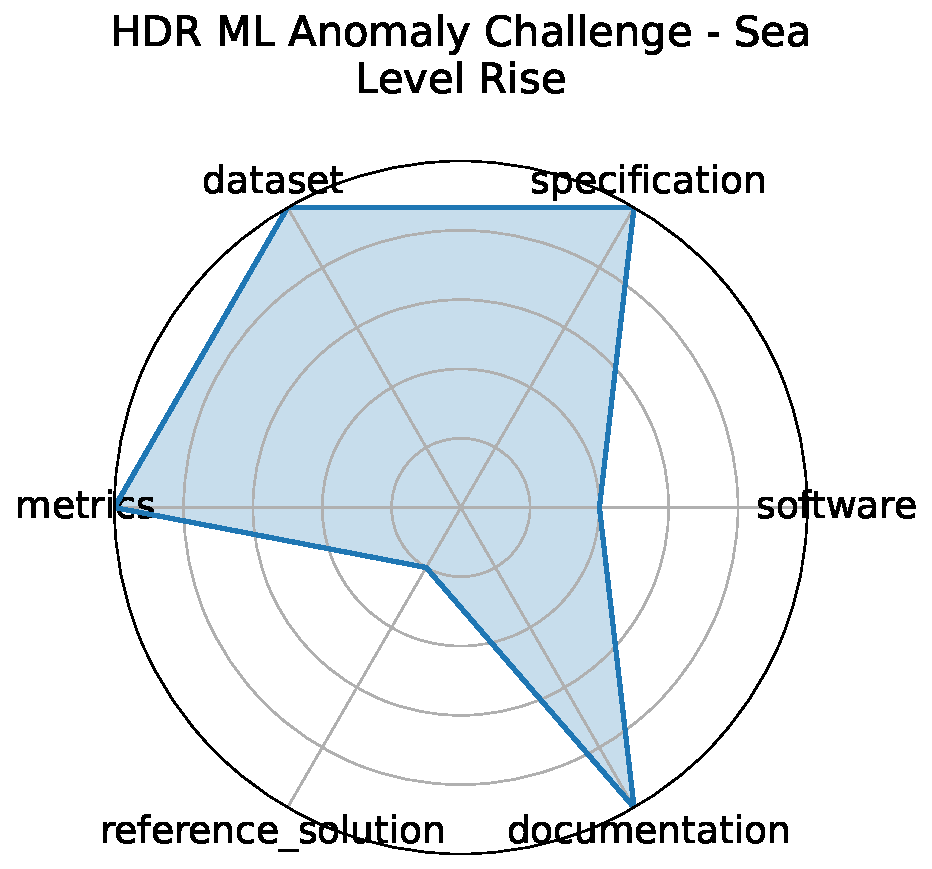
\includegraphics[width=0.15\textwidth]{hdr_ml_anomaly_challenge_-_sea_level_rise_radar.pdf} & HDR ML Anomaly Challenge - Sea Level Rise & Climate \& Earth Science & Detecting anomalous sea-level rise and flooding events via time-series and satellite imagery & anomaly detection, climate science, sea-level rise, time-series, remote sensing & Anomaly Detection & Anomaly Detection & Detection of environmental anomalies & ROC-AUC, Precision/Recall & CNNs, RNNs, Transformers & 3.83 & \cite{campolongo2025buildingmachinelearningchallenges3} \\ \hline
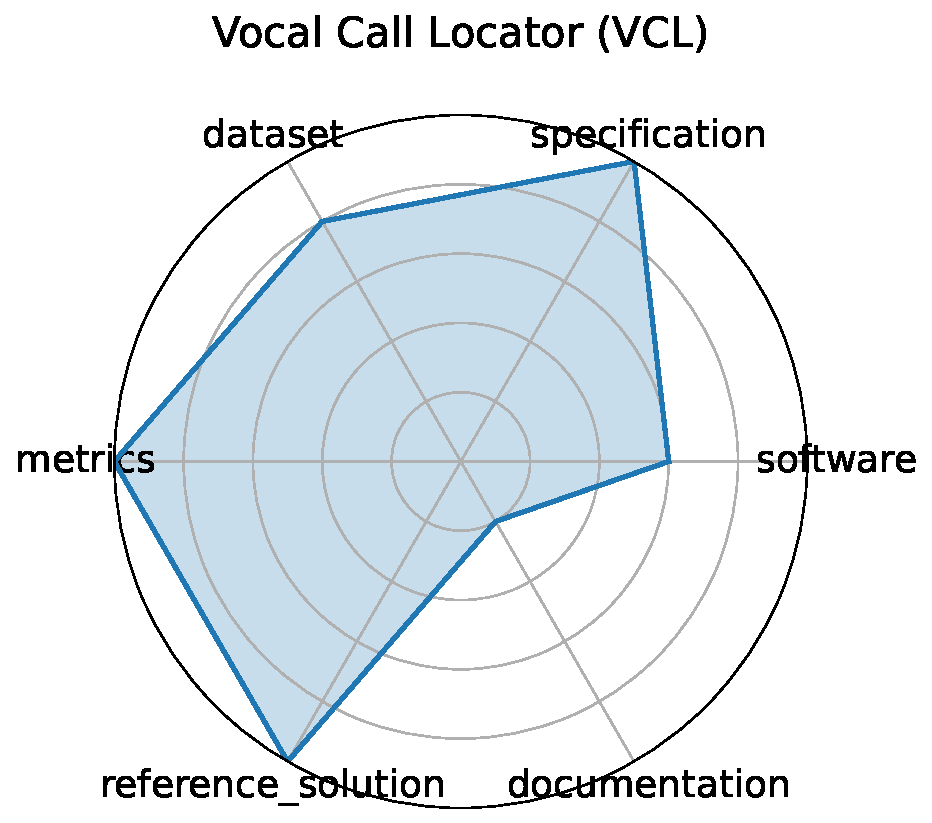
\includegraphics[width=0.15\textwidth]{vocal_call_locator_vcl_radar.pdf} & Vocal Call Locator (VCL) & Biology \& Medicine & Benchmarking sound-source localization of rodent vocalizations from multi-channel audio & source localization, bioacoustics, time-series, SSL & Sound source localization & Regression & Source localization accuracy in bioacoustic settings & Localization error (cm), Recall/Precision & CNN-based SSL models & 3.83 & \cite{neurips2024_c00d37d6} \\ \hline
\includegraphics[width=0.15\textwidth]{massspecgym_-_de_novo_molecule_generation_radar.pdf} & MassSpecGym - De novo molecule generation & Chemistry & Benchmark suite for discovery and identification of molecules via MS/MS & mass spectrometry, molecular structure, de novo generation, retrieval, dataset & De novo generation, Retrieval, Simulation & Generative & Molecular identification and generation from spectral data & Structure accuracy, Retrieval precision, Simulation MSE & Graph-based generative models, Retrieval baselines & 3.75 & \cite{neurips2024_c6c31413} \\ \hline
\includegraphics[width=0.15\textwidth]{massspecgym_-_molecule_retrieval_radar.pdf} & MassSpecGym - Molecule Retrieval & Chemistry & Benchmark suite for discovery and identification of molecules via MS/MS & mass spectrometry, molecular structure, de novo generation, retrieval, dataset & De novo generation, Retrieval, Simulation & Regression & Molecular identification and generation from spectral data & Structure accuracy, Retrieval precision, Simulation MSE & Graph-based generative models, Retrieval baselines & 3.75 & \cite{neurips2024_c6c31413} \\ \hline
\includegraphics[width=0.15\textwidth]{massspecgym_-_spectrum_simulation_radar.pdf} & MassSpecGym - Spectrum Simulation & Chemistry & Benchmark suite for discovery and identification of molecules via MS/MS & mass spectrometry, molecular structure, de novo generation, retrieval, dataset & De novo generation, Retrieval, Simulation & Regression & Molecular identification and generation from spectral data & Structure accuracy, Retrieval precision, Simulation MSE & Graph-based generative models, Retrieval baselines & 3.75 & \cite{neurips2024_c6c31413} \\ \hline
\includegraphics[width=0.15\textwidth]{spiqa_scientific_paper_image_question_answering_radar.pdf} & SPIQA (Scientific Paper Image Question Answering) & Computational Science \& AI & Multimodal QA on scientific figures & multimodal QA, figure understanding, table comprehension, chain-of-thought & Question answering, Multimodal QA, Chain-of-Thought evaluation & Multimodal Reasoning & Visual-textual reasoning in scientific contexts & Accuracy, F1 score & Chain-of-Thought models, Multimodal QA systems & 3.67 & \cite{zhong2024spiqa} \\ \hline
\includegraphics[width=0.15\textwidth]{gpqa_a_graduate-level_google-proof_question_and_answer_benchmark_radar.pdf} & GPQA: A Graduate-Level Google-Proof Question and Answer Benchmark & Biology \& Medicine, High Energy Physics, Chemistry & Graduate-level, expert-validated multiple-choice questions hard even with web access & Google-proof, multiple-choice, expert reasoning, science QA & Multiple choice & Reasoning \& Generalization & Scientific reasoning, knowledge probing & Accuracy & GPT-4 baseline & 3.67 & \cite{rein2023gpqagraduatelevelgoogleproofqa2} \\ \hline
\includegraphics[width=0.15\textwidth]{medqa_radar.pdf} & MedQA & Biology \& Medicine & Medical board exam QA & USMLE, diagnostic QA, medical knowledge, multilingual & Multiple choice & Reasoning \& Generalization & Medical diagnosis and knowledge retrieval & Accuracy & Neural reader, Retrieval-based QA systems & 3.50 & \cite{jin2020diseasedoespatienthave} \\ \hline
\includegraphics[width=0.15\textwidth]{single_qubit_readout_on_qick_system_radar.pdf} & Single Qubit Readout on QICK System & Computational Science \& AI & Real-time single-qubit state classification using FPGA firmware & qubit readout, hls4ml, FPGA, QICK & Classification & Classification & Single-shot fidelity, inference latency & Accuracy, Latency & hls4ml quantized NN & 3.50 & \cite{diguglielmo2025endtoendworkflowmachinelearningbased} \\ \hline
\includegraphics[width=0.15\textwidth]{cfdbench_fluid_dynamics_radar.pdf} & CFDBench (Fluid Dynamics) & Mathematics & Neural operator surrogate modeling & neural operators, CFD, FNO, DeepONet & Surrogate modeling & Regression & Generalization of neural operators for PDEs & L2 error, MAE & FNO, DeepONet, U-Net & 3.33 & \cite{luo2024cfdbenchlargescalebenchmarkmachine} \\ \hline
\includegraphics[width=0.15\textwidth]{curie_scientific_long-context_understanding_reasoning_and_information_extraction_radar.pdf} & CURIE (Scientific Long-Context Understanding, Reasoning and Information Extraction) & Materials Science, High Energy Physics, Biology \& Medicine, Chemistry, Climate \& Earth Science & Long-context scientific reasoning & long-context, information extraction, multimodal & Information extraction, Reasoning, Concept tracking, Aggregation, Algebraic manipulation, Multimodal comprehension & Reasoning \& Generalization & Long-context understanding and scientific reasoning & Accuracy & unkown & 3.33 & \cite{cui2025curieevaluatingllmsmultitask} \\ \hline
\includegraphics[width=0.15\textwidth]{smart_pixels_for_lhc_radar.pdf} & Smart Pixels for LHC & High Energy Physics & On-sensor, in-pixel ML filtering for high-rate LHC pixel detectors & smart pixel, on-sensor inference, data reduction, trigger & Image Classification, Data filtering & Classification & On-chip, low-power inference; data reduction & Data rejection rate, Power per pixel & 2-layer pixel NN & 3.33 & \cite{parpillon2024smartpixelsinpixelai} \\ \hline
\includegraphics[width=0.15\textwidth]{lhc_new_physics_dataset_radar.pdf} & LHC New Physics Dataset & High Energy Physics & Real-time LHC event filtering for anomaly detection using proton collision data & anomaly detection, proton collision, real-time inference, event filtering, unsupervised ML & Anomaly Detection, Event classification & Anomaly Detection & Unsupervised signal detection under latency and bandwidth constraints & ROC-AUC, Detection efficiency & Autoencoder, Variational autoencoder, Isolation forest & 3.33 & \cite{https://doi.org/10.5281/zenodo.5046389} \\ \hline
\includegraphics[width=0.15\textwidth]{quantum_computing_benchmarks_qml_radar.pdf} & Quantum Computing Benchmarks (QML) & Computational Science \& AI & Quantum algorithm performance evaluation & quantum circuits, state preparation, error correction & Circuit benchmarking, State classification & Classification & Quantum algorithm performance and fidelity & Fidelity, Success probability & IBM Q, IonQ, AQT@LBNL & 3.17 & \cite{bowles2024betterclassicalsubtleart} \\ \hline
\includegraphics[width=0.15\textwidth]{ultrafast_jet_classification_at_the_hl-lhc_radar.pdf} & Ultrafast jet classification at the HL-LHC & High Energy Physics & FPGA-optimized real-time jet origin classification at the HL-LHC & jet classification, FPGA, quantization-aware training, Deep Sets, Interaction Networks & Classification & Classification & Real-time inference under FPGA constraints & Accuracy, Latency, Resource utilization & MLP, Deep Sets, Interaction Network & 3.17 & \cite{odagiu2024ultrafastjetclassificationfpgas} \\ \hline
\includegraphics[width=0.15\textwidth]{hedm_braggnn_radar.pdf} & HEDM (BraggNN) & Materials Science & Fast Bragg peak analysis using deep learning in diffraction microscopy & BraggNN, diffraction, peak finding, HEDM & Peak detection & Classification & High-throughput peak localization & Localization accuracy, Inference time & BraggNN & 3.17 & \cite{liu2021braggnnfastxraybragg} \\ \hline
\includegraphics[width=0.15\textwidth]{d-stem_radar.pdf} & 4D-STEM & Materials Science & Real-time ML for scanning transmission electron microscopy & 4D-STEM, electron microscopy, real-time, image processing & Image Classification, Streamed data inference & Classification & Real-time large-scale microscopy inference & Classification accuracy, Throughput & CNN models (prototype) & 3.17 & \cite{qin2023extremely} \\ \hline
\includegraphics[width=0.15\textwidth]{beam_control_radar.pdf} & Beam Control & High Energy Physics & Reinforcement learning control of accelerator beam position & RL, beam stabilization, control systems, simulation & Control & Reinforcement Learning/Control & Policy performance in simulated accelerator control & Stability, Control loss & DDPG, PPO (planned) & 3.00 & \cite{duarte2022fastmlsciencebenchmarksaccelerating3,kafkes2021boostrdatasetacceleratorcontrol} \\ \hline
\includegraphics[width=0.15\textwidth]{intelligent_experiments_through_real-time_ai_radar.pdf} & Intelligent experiments through real-time AI & High Energy Physics & Real-time FPGA-based triggering and detector control for sPHENIX and future EIC & FPGA, Graph Neural Network, hls4ml, real-time inference, detector control & Trigger classification, Detector control, Real-time inference & Classification & Low-latency GNN inference on FPGA & Accuracy (charm and beauty detection), Latency (micros), Resource utilization (LUT/FF/BRAM/DSP) & Bipartite Graph Network with Set Transformers (BGN-ST), GarNet (edge-classifier) & 3.00 & \cite{kvapil2025intelligentexperimentsrealtimeai} \\ \hline
\includegraphics[width=0.15\textwidth]{hdr_ml_anomaly_challenge_-_butterfly_radar.pdf} & HDR ML Anomaly Challenge - Butterfly & Biology \& Medicine & Detecting hybrid butterflies via image anomaly detection in genomic-informed dataset & anomaly detection, computer vision, genomics, butterfly hybrids & Anomaly Detection & Anomaly Detection & Hybrid detection in biological systems & Classification accuracy, F1 score & CNN-based detectors & 3.00 & \cite{campolongo2025buildingmachinelearningchallenges2} \\ \hline
\includegraphics[width=0.15\textwidth]{dune_radar.pdf} & DUNE & High Energy Physics & Real-time ML for DUNE DAQ time-series data & DUNE, time-series, real-time, trigger & Trigger selection, Time-series anomaly detection & Anomaly Detection & Low-latency event detection & Detection efficiency, Latency & CNN, LSTM (planned) & 2.83 & \cite{abud2021deep} \\ \hline
\includegraphics[width=0.15\textwidth]{frontiermath_radar.pdf} & FrontierMath & Mathematics & Challenging advanced mathematical reasoning & symbolic reasoning, number theory, algebraic geometry, category theory & Problem solving & Reasoning \& Generalization & Symbolic and abstract mathematical reasoning & Accuracy & unknown & 2.50 & \cite{glazer2024frontiermathbenchmarkevaluatingadvanced} \\ \hline
\includegraphics[width=0.15\textwidth]{aime_american_invitational_mathematics_examination_radar.pdf} & AIME (American Invitational Mathematics Examination) & Mathematics & Pre-college advanced problem solving & algebra, combinatorics, number theory, geometry & Problem solving & Reasoning \& Generalization & Mathematical problem-solving and reasoning & Accuracy & unknown & 2.33 & \cite{www-aime} \\ \hline
\includegraphics[width=0.15\textwidth]{quench_detection_radar.pdf} & Quench detection & High Energy Physics & Real-time detection of superconducting magnet quenches using ML & quench detection, autoencoder, anomaly detection, real-time & Anomaly Detection, Quench localization & Anomaly Detection & Real-time anomaly detection with multi-modal sensors & ROC-AUC, Detection latency & Autoencoder, RL agents (in development) & 2.17 & \cite{quench2024} \\ \hline
\includegraphics[width=0.15\textwidth]{materials_project_radar.pdf} & Materials Project & Materials Science & DFT-based property prediction & DFT, materials genome, high-throughput & Property prediction & Regression & Prediction of inorganic material properties & MAE, R{\textasciicircum}2 & Automatminer, Crystal Graph Neural Networks & 1.92 & \cite{jain2013materials} \\ \hline
\includegraphics[width=0.15\textwidth]{in-situ_high-speed_computer_vision_radar.pdf} & In-Situ High-Speed Computer Vision & High Energy Physics & Real-time image classification for in-situ plasma diagnostics & plasma, in-situ vision, real-time ML & Image Classification & Classification & Real-time diagnostic inference & Accuracy, FPS & CNN & 1.50 & \cite{wei2024lowlatencyopticalbasedmode} \\ \hline
\end{longtable}
}

\end{landscape}
